%\documentclass[12pt,twoside,onecolumn,letterpaper]{article}
%\documentclass[12pt,twoside,onecolumn,letterpaper]{article}
%\documentclass[10pt,oneside,onecolumn,letterpaper]{article}
\usepackage[spanish]{babel}
\usepackage[utf8]{inputenc}
\usepackage{hyperref}
\usepackage{graphicx}
\usepackage{fancyhdr}
\usepackage{enumerate}
\usepackage{color}
\usepackage{colortbl}
\definecolor{gray}{cmyk}{0.0,0.0,0.0,0.60}
 
\mode<article>{
\hoffset-25mm
\voffset-25mm
%\marginparwidth=0mm
%\marginparsep=0mm
\headheight=16pt
\oddsidemargin=25mm
\evensidemargin=25mm
\textwidth=165mm
\topmargin=20mm
\textheight=220mm

\pagestyle{fancy}
\fancyhf{}
\fancyhead[RO]{\small{\textcolor{gray}{\textsc{Propuesta de investgaci\'on: Locomoci\'on b\'ipeda ...}}}}
\fancyhead[LO]{
\includegraphics[scale=0.05]{../images/unlogo.png}}
\fancyhead[LE]{
\includegraphics[scale=0.05]{../images/unlogo.png}\quad\small{\textcolor{gray}{\textsc{Doctorado en ingenieria: Mecanica y Mecatronica}}}}
\fancyfoot[CO,CE]{\thepage}
\fancyfoot[LO,RE]{\scriptsize{\textcolor{gray}{\emph{Version 0.4}}}}
}

\mode<article>{
\title{
\includegraphics[scale=0.15]{../images/unescudobn.png}\\\vspace{-0.2cm}
  \textsc{\underline{\small{Universidad Nacional de Colombia}}\\\tiny{Sede Bogot\'a}\\\small{Facultad de Ingenier\'ia\\\vspace{-0.2cm}Unidad de Posgrado}}\\\vspace{0.5cm}
       \LARGE \textbf{Locomoci\'on de caminadores b\'ipedos: Rob\'otica subactuada, control, planeaci\'on, dise\~no y aplicaciones}}
\author{J.A. Castillo Le\'on \thanks{jacastillol@unal.edu.co}}
}
\mode<presentation>{
\usepackage{xcolor}
\definecolor{blueun}{rgb}{0.047,0.294,0.376}
\usepackage{multimedia}
\usepackage{animate}

%%%% BEGINT TIME LINE +++++++++++++++++++++++++++++++++++++++++++++++++++++++++++
\usepackage{ifthen}
\usepackage[firstyear=1999,lastyear=2012]{moderntimeline}

\makeatletter
% change these colors according to your needs
\colorlet{color0}{blue}
\colorlet{color1}{olive}

\newcommand*{\hintfont}{}
\newcommand*{\hintstyle}[1]{{\hintfont\textcolor{color0}{#1}}}
\newcommand*{\listitemsymbol}{a~}
\newcommand*{\cventry}[7][.25em]{%
  \cvitem[#1]{#2}{%
    {\bfseries\raggedright #3}%
    \ifthenelse{\equal{#4}{}}{}{, \raggedright{\slshape#4}}%
    \ifthenelse{\equal{#5}{}}{}{,  \raggedright#5}%
    \ifthenelse{\equal{#6}{}}{}{, \raggedright#6}%
    .\strut%
    \ifx&#7&%
      \else{\newline{}\begin{minipage}[t]{\linewidth}\small\raggedright#7\end{minipage}}\fi}}
\newcommand*{\cvitem}[3][.25em]{%
  \begin{tabular}{@{}p{\hintscolumnwidth}@{\hspace{\separatorcolumnwidth}}p{\maincolumnwidth}@{}}%
      \raggedleft\hintstyle{#2} & {#3}%
  \end{tabular}%
  \par\addvspace{#1}}
\tlmaxdates{2001}{2012}
\newlength{\quotewidth}
\newlength{\hintscolumnwidth}
\setlength{\hintscolumnwidth}{0.175\textwidth}
\newlength{\separatorcolumnwidth}
\setlength{\separatorcolumnwidth}{0.025\textwidth}
\newlength{\maincolumnwidth}
\newlength{\doubleitemmaincolumnwidth}
\newlength{\listitemsymbolwidth}
\settowidth{\listitemsymbolwidth}{\listitemsymbol}
\newlength{\listitemmaincolumnwidth}
\newlength{\listdoubleitemmaincolumnwidth}

\setlength{\maincolumnwidth}{\dimexpr0.9\linewidth-\separatorcolumnwidth-\hintscolumnwidth\relax}
\makeatother
%%%% END TIME LINE +++++++++++++++++++++++++++++++++++++++++++++++++++++++++++

\usetheme[secheader]{PaloAlto}%PaloAlto,Marburg,Hannover
\usecolortheme[RGB={12,75,96}]{structure}%beetle,albatross,structure
\logo{
\includegraphics[height=1.45cm]{../images/unescudo.png}}
\title[Locomoci\'on b\'ipeda ...]{\textbf{Locomoci\'on de caminadores b\'ipedos: Rob\'otica subactuada, control, planeaci\'on, dise\~no y aplicaciones}}
\author[J.A. Castillo Le\'on]{\textbf{Proponente:} Jaime Andr\'es Castillo Le\'on\inst{1} \and \\\textbf{Director:} PhD. Ing. Ricardo Ram\'irez Heredia\inst{1}}
\institute[UN]{\inst{1}Departamento de Ingenier\'ia Mec\'anica y Mecatr\'onica \\Universidad Nacional de Colombia}
}
\date{}

\begin{document}

\renewcommand{\tablename}{Tabla}

\maketitle
\mode<presentation>{
\begin{frame}
  \titlepage
  \frametitle{Propuesta de Investigaci\'on}
\end{frame}
}
{\large\textbf{Director de investigaci\'on:} PhD. Ing. Ricardo Ram\'irez Heredia}\par\vspace{0.7cm}
{\large\textbf{L\'inea de investigaci\'on:} Rob\'otica}

%\mode<all>
%\mode*
% Plataformas e instituciones:
% USA-MIT-Tedrake-TODDLER
% RABBIT-EMARO-Universidad de Nantes-
\section[Justificaci\'on]{Justificaci\'on}
\label{sec:justify}

\mode<presentation>{
\begin{frame}
  \frametitle{Por qu\'e esta investigaci\'on?}
  \framesubtitle{Universidades, Institutos, Centros y Laboratorios trabajando en Rob\'otica B\'ipeda}
  \begin{center}
    \includegraphics[height=7cm]{../images/BipedInstitutesAndUniversities.png}
  \end{center}
\end{frame}
\begin{frame}
  \frametitle{Por qu\'e esta investigaci\'on?}
  \framesubtitle{Algunas plataformas b\'ipedas}
  \begin{center}
    \includegraphics[height=6.5cm]{../images/BipedPlatforms.png}
  \end{center}
\end{frame}
\begin{frame}[label=def_multi]
  \frametitle{Por qu\'e esta investigaci\'on?}
  \framesubtitle{Trabajo multidisciplinario}
  \begin{center}
    \only<1-6,7>{
      \only<1-6>{\vspace{-2.0cm}}
      \only<7>{\vspace{-0.3cm}}
      \begin{columns}[c]
        \begin{column}{3cm}
          \only<1>{\setbeamercolor{postit}{fg=white,bg=red!50!black}}
          \only<2-7>{\setbeamercolor{postit}{fg=white,bg=red}}
          \hyperlink{exp_embebidos}{
          \begin{beamercolorbox}[sep=0.5em,wd=3cm,rounded=true,center,shadow=true]{postit}
            \only<1>{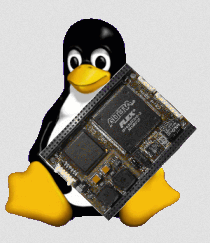
\includegraphics[height=1.5cm]{../images/ThemeEmbedded.png}\\}
            \only<2-6>{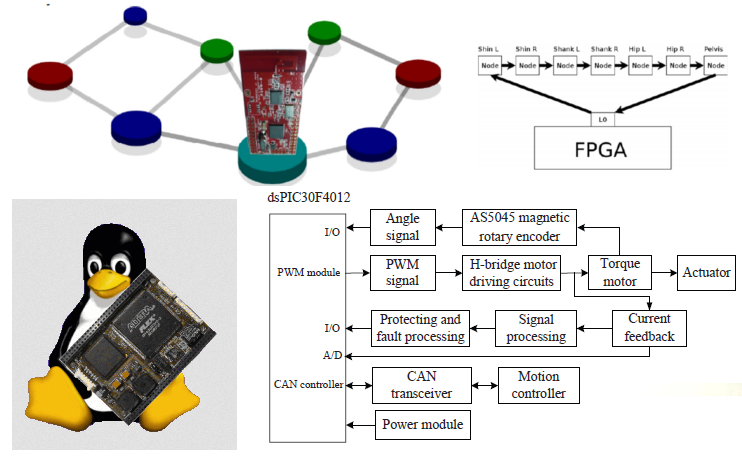
\includegraphics[height=1.5cm]{../images/ShortEmbedded.png}\\}
            \textbf{Sistemas Embebidos}
          \end{beamercolorbox}}
        \end{column}
        \begin{column}{3cm}
          \only<1-2>{\setbeamercolor{postit}{fg=white,bg=yellow!70!black}}
          \only<3-7>{\setbeamercolor{postit}{fg=white,bg=yellow}}
          \hyperlink{exp_biomecanica}{
          \begin{beamercolorbox}[sep=0.5em,wd=3cm,rounded=true,center,shadow=true]{postit}
            \only<1-2>{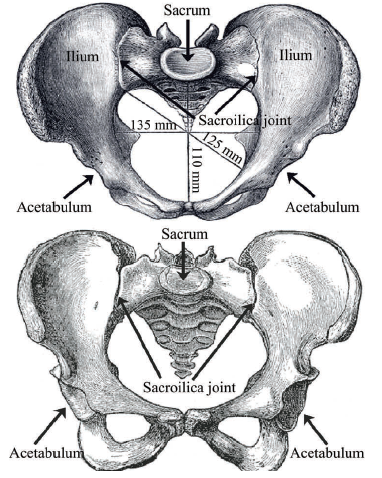
\includegraphics[height=1.5cm]{../images/ThemeBiomechanics.png}\\}
            \only<3-6>{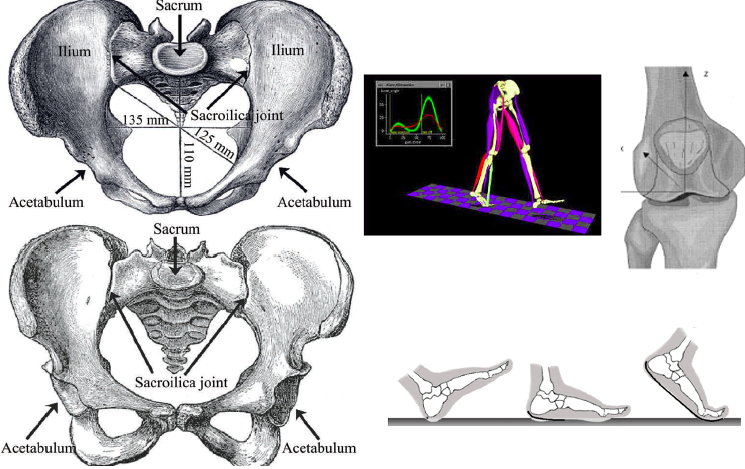
\includegraphics[height=1.5cm]{../images/ShortBiomechanics.png}\\}
            \textbf{Biomec\'anica}
          \end{beamercolorbox}}
        \end{column}
        \begin{column}{3cm}
          \only<1-3>{\setbeamercolor{postit}{fg=white,bg=blue!50!black}}
          \only<4-7>{\setbeamercolor{postit}{fg=white,bg=blue}}
          \hyperlink{exp_mecanismos}{
          \begin{beamercolorbox}[sep=0.5em,wd=3cm,rounded=true,center,shadow=true]{postit}
            \only<1-3>{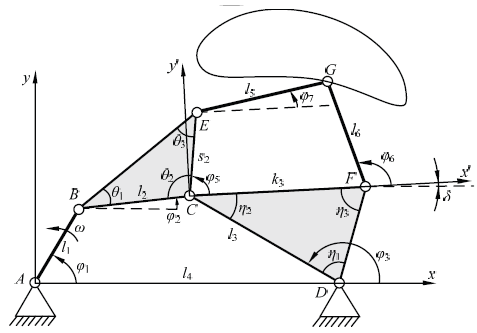
\includegraphics[height=1.5cm]{../images/ThemeMechanisms.png}\\}
            \only<4-6>{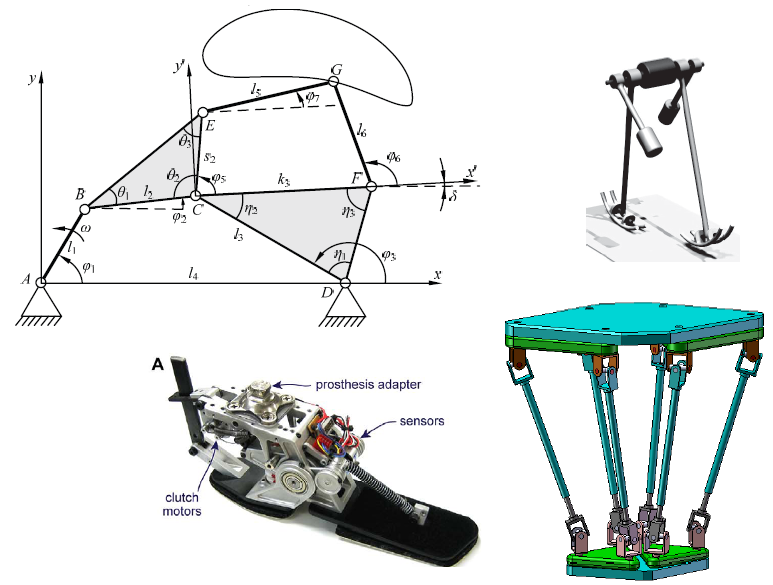
\includegraphics[height=1.5cm]{../images/ShortMechanisms.png}\\}
            \textbf{Modelado y Mecanismos}
          \end{beamercolorbox}}
        \end{column}
      \end{columns}
      \vspace{1.0cm}
      \begin{columns}[c]
        \begin{column}{3cm}
          \only<1-4>{\setbeamercolor{postit}{fg=white,bg=black}}
          \only<5-7>{\setbeamercolor{postit}{fg=white,bg=white!50!black}}
          \hyperlink{exp_computacion_flexible}{
          \begin{beamercolorbox}[sep=0.5em,wd=3cm,rounded=true,center,shadow=true]{postit}
            \textbf{C. Flexible y Optimizaci\'on}
            \only<1-4>{\\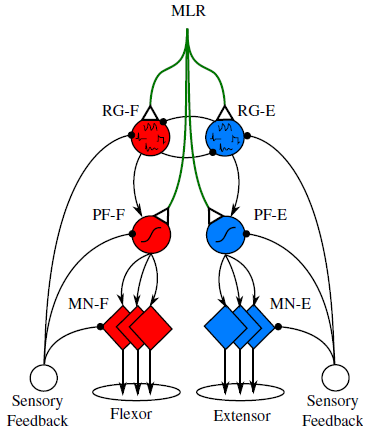
\includegraphics[height=1.5cm]{../images/ThemeSoftComputing.png}}
            \only<5-6>{\\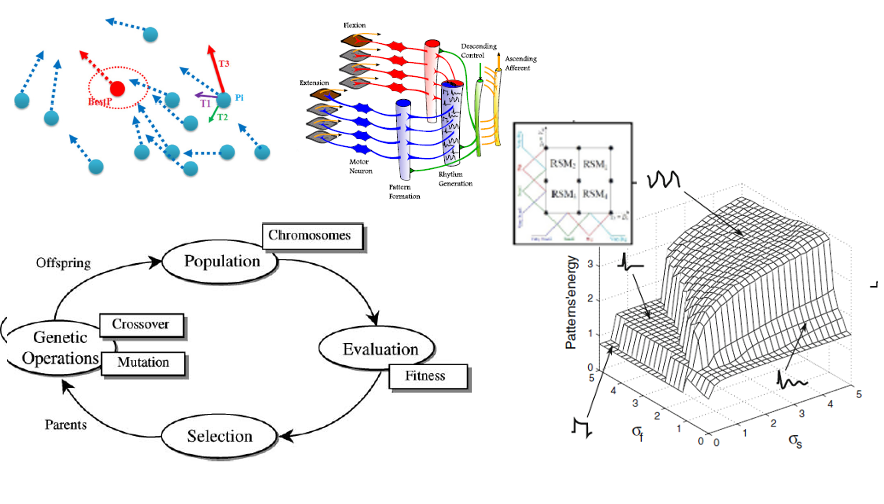
\includegraphics[height=1.5cm]{../images/ShortSoftComputing.png}}
          \end{beamercolorbox}}
        \end{column}
        \begin{column}{3cm}
          \only<1-5>{\setbeamercolor{postit}{fg=white,bg=green!50!black}}
          \only<6-7>{\setbeamercolor{postit}{fg=white,bg=green}}
          \hyperlink{exp_control}{
          \begin{beamercolorbox}[sep=0.5em,wd=3cm,rounded=true,center,shadow=true]{postit}
            \textbf{Control y Sis. Din\'amicos}
            \only<1-5>{\\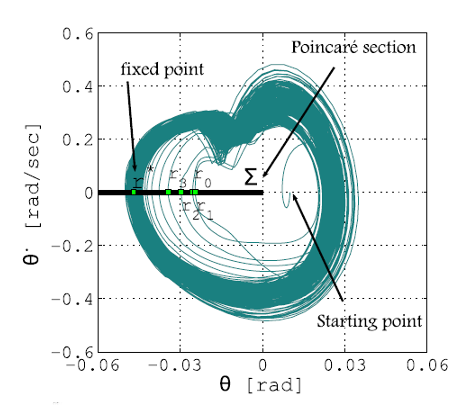
\includegraphics[height=1.5cm]{../images/ThemeControl.png}}
            \only<6-6>{\\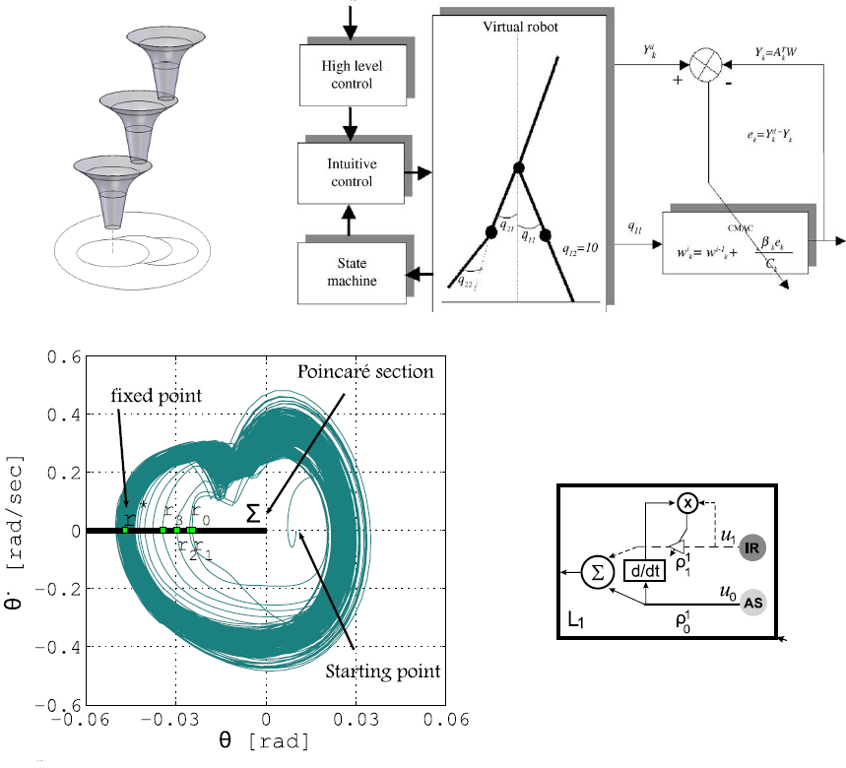
\includegraphics[height=1.5cm]{../images/ShortControl.png}}
          \end{beamercolorbox}}
        \end{column}
      \end{columns}
      \only<1-6>{\vspace{-4.6cm}}
      \only<7>{\vspace{-3.1cm}}
      \hspace{-0.1cm}
      \setbeamercolor{postit}{fg=white,bg=blueun}
      \begin{beamercolorbox}[sep=0.5em,wd=4.0cm,rounded=true,center]{postit}
        \textbf{\Large\textcolor{white}{ROB\'OTICA B\'IPEDA}}
      \end{beamercolorbox}
    }
%    \only<2>{\textbf{\textcolor{blueun}{Sistemas Embebidos}}\\
%    \includegraphics[height=6.5cm]{../images/Embedded.png}}
%    \only<3>{\textbf{\textcolor{blueun}{Biomec\'anica}}\\
%    \includegraphics[height=5.8cm]{../images/Biomechanics.png}}
%    \only<4>{\textbf{\textcolor{blueun}{Modelado de sistemas mec\'anicos y s\'intesis de mecanismos}}\\
%    \includegraphics[height=6.0cm]{../images/Mechanisms.png}}
%    \only<5>{\textbf{\textcolor{blueun}{Optimizaci\'on, computaci\'on flexible e IA}}\\
%    \includegraphics[height=6.0cm]{../images/SoftComputing.png}}
%    \only<6>{\textbf{\textcolor{blueun}{Control}}\\
%    \includegraphics[height=6.5cm]{../images/Control.png}}
  \end{center}
\end{frame}
\begin{frame}
  \frametitle{Por qu\'e esta investigaci\'on?}
  \framesubtitle{Algunos aspecto para la justificaci\'on}
  \quad\hspace{-0.8cm}\makebox{
    \begin{columns}[T]
      \small
      \begin{column}{6cm}
        \begin{enumerate}
        \item Como ayuda de la proliferaci\'on
          \only<2-6>{
            \begin{itemize}\scriptsize
            \item<2-> Bajo costo
            \item<3-> Didacticos
            \item<4-> Modularidad
            \item<5-> Prototipado rapido
            \item<6-> Metodologia de dise\~no
            \end{itemize}
          }
        \item<7-> Motivaci\'on personal
        \item<8-> Posibles productos y soluciones
          \only<9-13>{
            \begin{itemize}\scriptsize
            \item<9-> Teleoperaci\'on
            \item<10-> Manufactura, transporte y ensambles
            \item<11-> Movilidad en cuadrapl\'ejicos, pr\'otesis y caminata pasiva
            \item<12-> Educaci\'on, cursos y materias
            \item<13-> Entretenimiento e IA
            \end{itemize}
          }
        \item<14-> Viabilidad
          \only<15->{
            \begin{itemize}\scriptsize
            \item<15-> Recursos f\'isicos
            \item<16-> Profesores, grupos de investigaci\'on y materias
            \item<17-> Concursos para recursos economicos y de financiaci\'on
            \item<18-> Relaciones con grupos internacionales de investigaci\'on
            \item<19-> Experiencia del director de investigaci\'on en el tema
            \item<20-> Experiencia del investigador en el proyecto
            \end{itemize}
          }
        \end{enumerate}
      \end{column}
      \begin{column}{4cm}
        % \fbox{
        \parbox[c][7cm][c]{4cm}{
          \only<1-4>{
            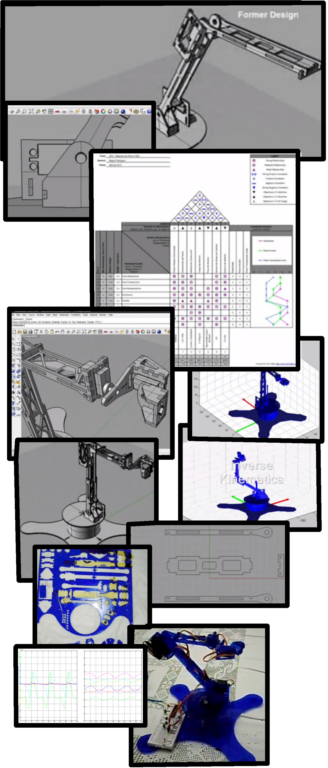
\includegraphics[height=7cm]{../images/RobotMR1_0.png}
          }
          \only<5>{
            %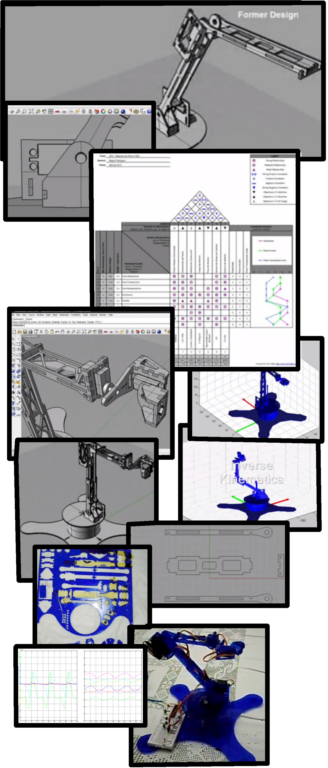
\includegraphics[height=7cm]{../images/RobotMR1_0.png}
            \animategraphics[height=7cm,autoresume,autoplay,loop]{2}{../images/RobotMR1_}{0}{12}
          }
          \only<6>{
            %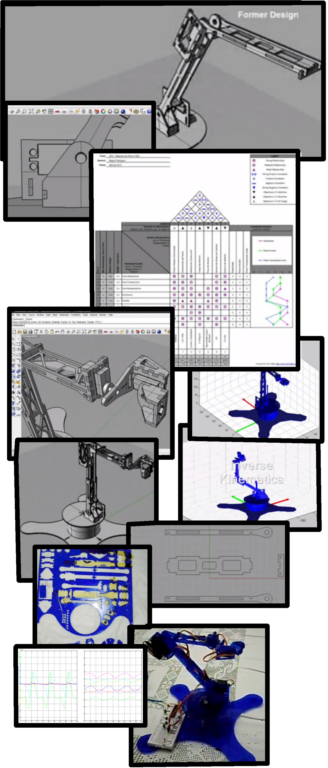
\includegraphics[height=7cm]{../images/RobotMR1_0.png}
            \movie[width=3cm,height=7cm,externalviewer]{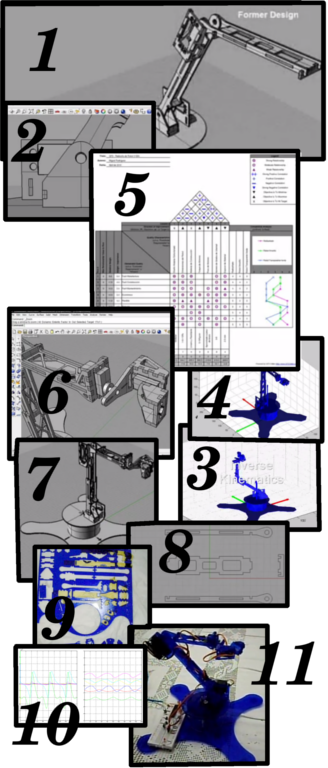
\includegraphics[height=7cm]{../images/RobotMR1_12.png}}{../videos/RobotMR1.flv} 
          }
          \only<7>{
            Ponga algo que haya hecho!!
          }
          \only<9>{
            \scriptsize
            Teleoperaci\'on
            \begin{center}
              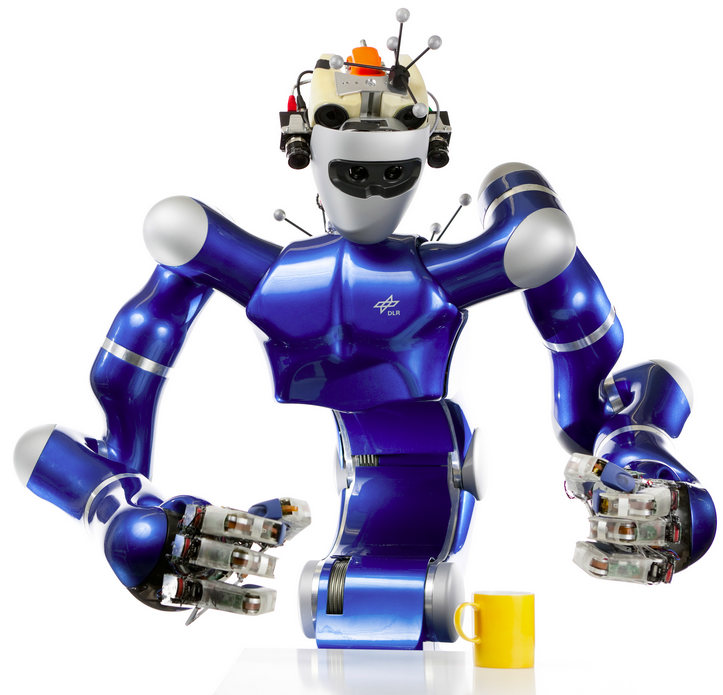
\includegraphics[width=4.0cm]{../images/Teleoperacion.png}
            \end{center}
          }
          \only<10>{
            \scriptsize
            Transporte
            \begin{center}
              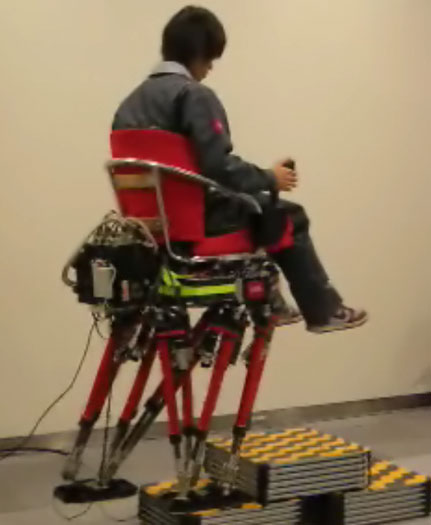
\includegraphics[width=4.0cm]{../images/Transporte.png}
            \end{center}
          }
          \only<11>{
            \scriptsize
            Biomec\'anica
            \begin{center}
              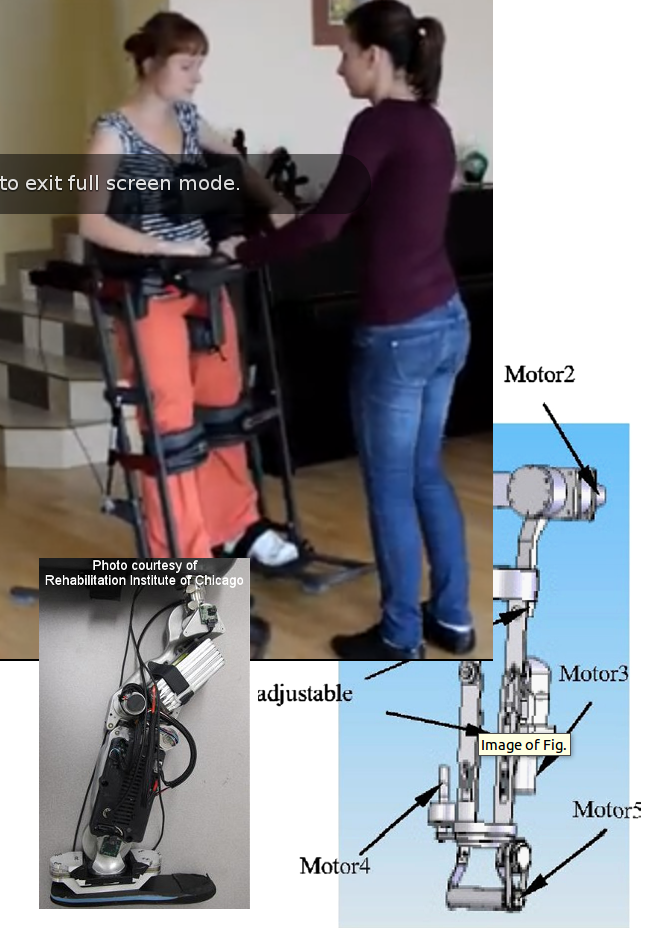
\includegraphics[width=4.0cm]{../images/ProsthesisAndPhysiotherapy.png}
            \end{center}
          }
          \only<12>{
            \scriptsize
            Educaci\'on
            \begin{center}
              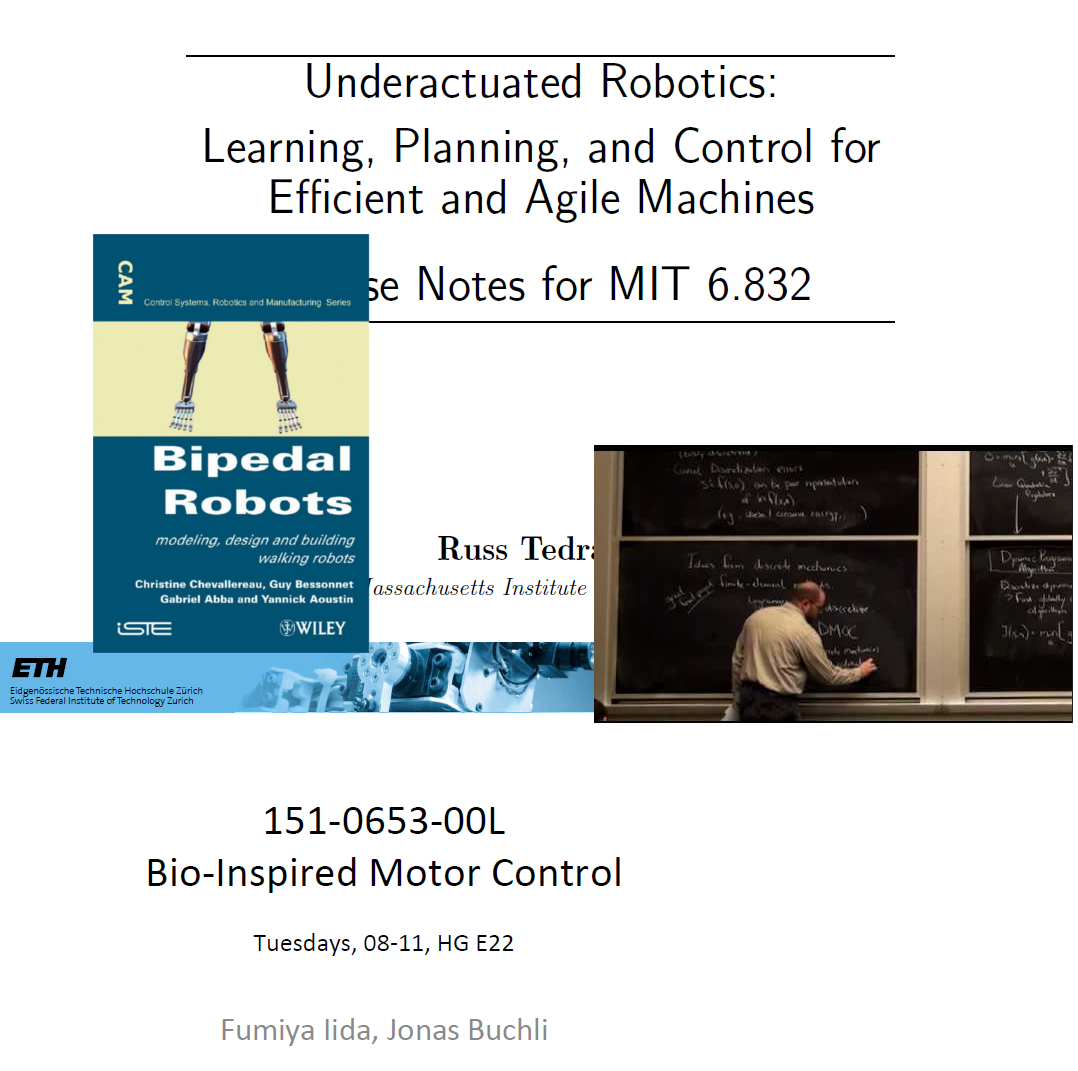
\includegraphics[width=4.0cm]{../images/Educacion.png}
            \end{center}
          }
          \only<13>{
            \scriptsize
            Entretenimiento
            \begin{center}
              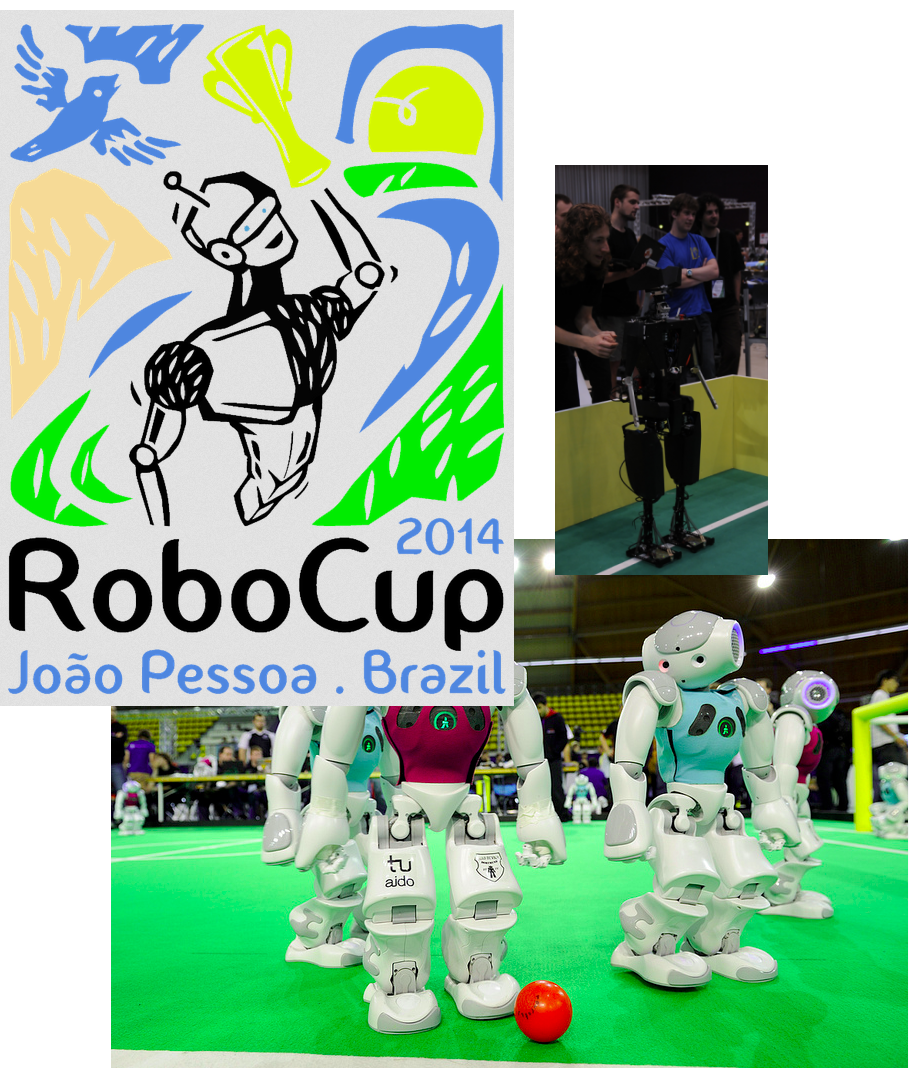
\includegraphics[width=4.0cm]{../images/Entretenimiento.png}
            \end{center}
          }
          \only<15>{
            \scriptsize
            \begin{itemize}
            \item CNC
            \item Impresoras 3D
            \item Software CAD-CAM-CAE
            \item Laboratorios con plataformas
            \end{itemize}
          }
          \only<16>{
            \scriptsize
            \begin{itemize}
            \item Din\'amica de robots (R. Ram\'irez)
            \item Biomec\'anica (D. Garzon)
            \item Sistemas embebidos (C. Camargo)
            \item Control de robots (J. Sofrony)
            \item Aprendizaje de m\'aquina (F. Gonz\'alez)
            \item Optimizaci\'on (A. Tovar)
            \item Computaci\'on flexible (L.F Ni\~no)
            \item Inteligencia Artificial (J. G\'omez)
            \end{itemize}
          }
          \only<18>{
            \scriptsize
            \begin{itemize}
            \item Justin DLR (M. Roa)
            \item Robonaut 2 GM-NASA (L. Barajas)
            \item Walking Dynamics Conferences
            \end{itemize}
          }
          \only<19>{
            \scriptsize
            \begin{center}
              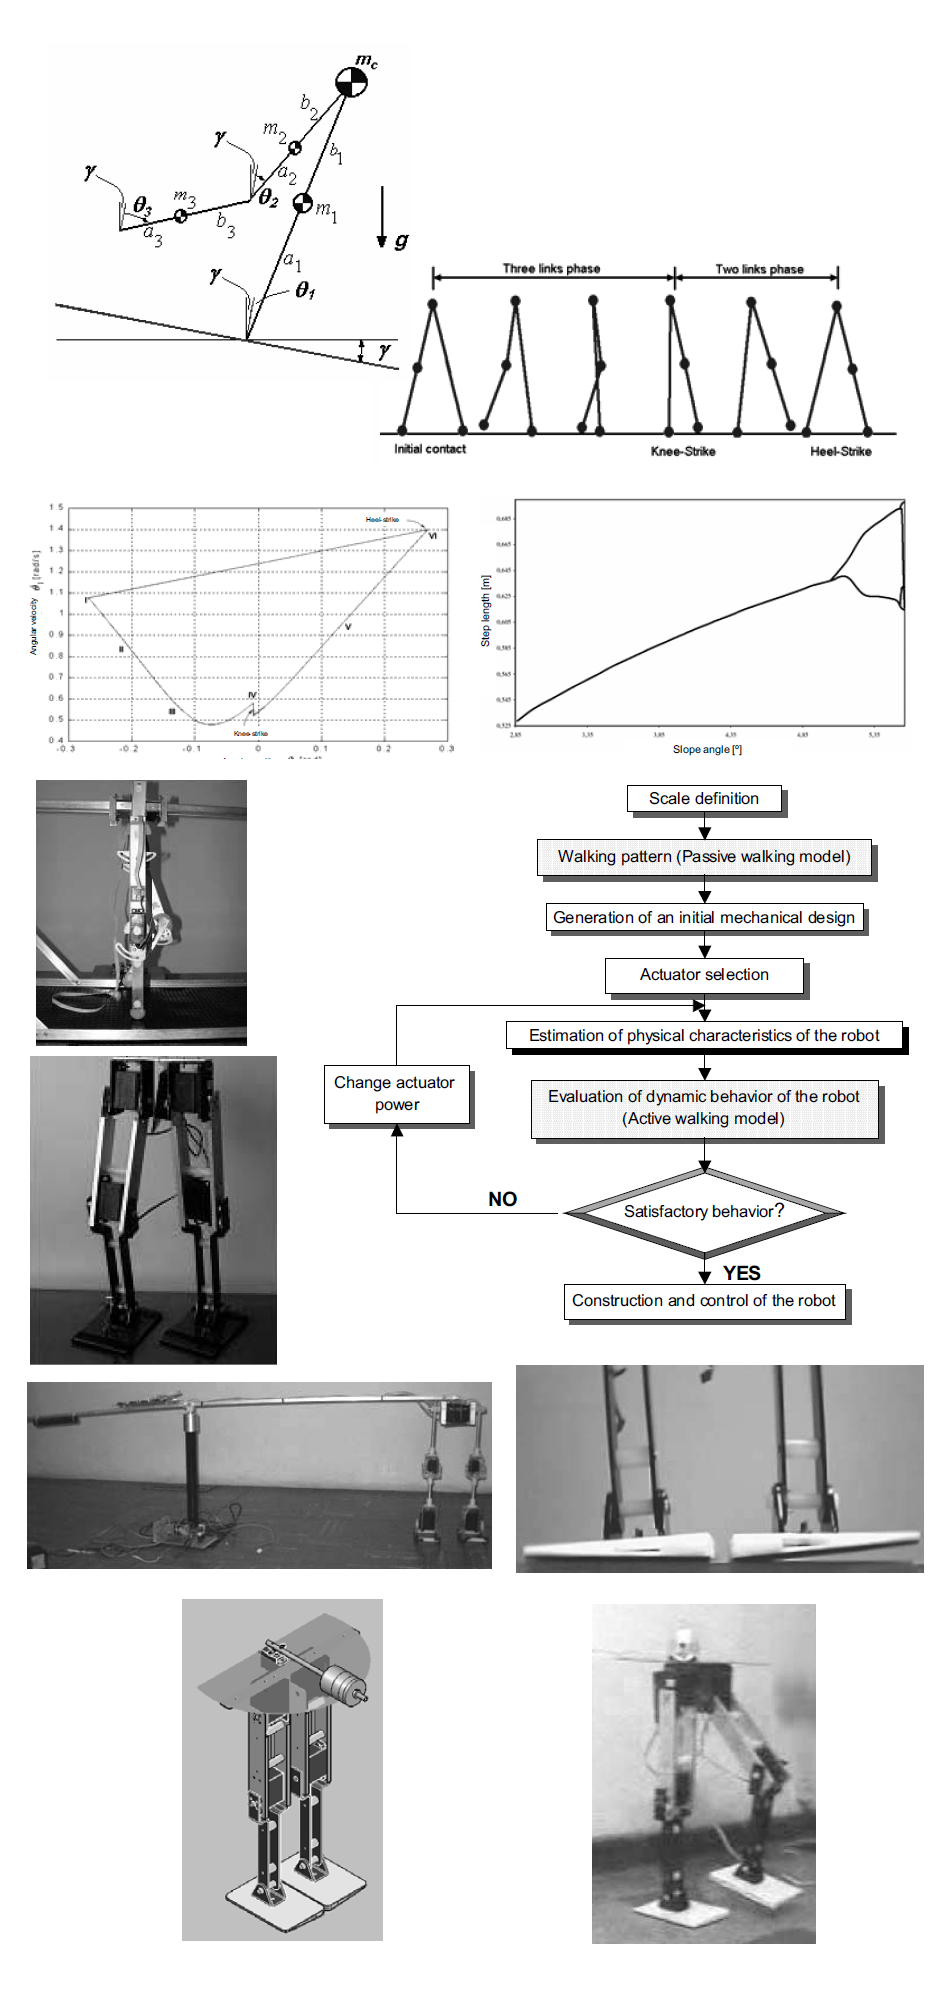
\includegraphics[height=7.0cm]{../images/UNROCA.png}
            \end{center}
          }
          \only<20>{
            \scriptsize
            \begin{center}%P1(120,360),P2(1110,530)
              %\includegraphics[height=7cm]{../images/SomeThingsByMe_0.png}
              \animategraphics[height=7cm,loop]{1}{../images/SomeThingsByMe_}{1}{5}
            \end{center}
          }
        }
        % }
      \end{column}
    \end{columns}
  }
  \only<18>{\vspace{-2.0cm}
    \begin{center}
      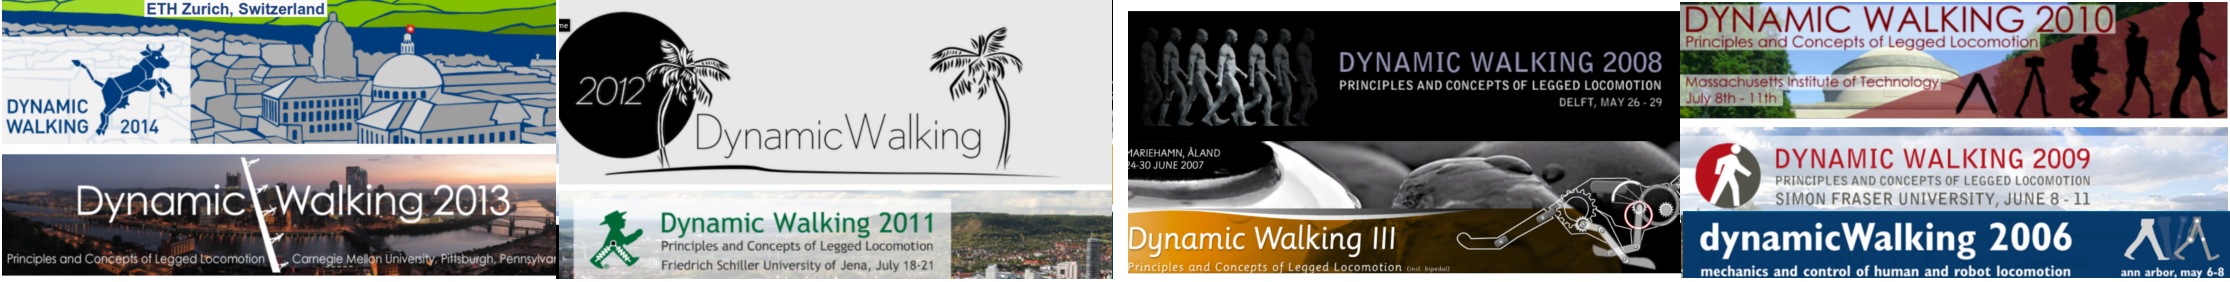
\includegraphics[width=10.0cm]{../images/DynamicWalkingConferences.png}
    \end{center}
  }
\end{frame}
\begin{frame}
  \frametitle{Por qu\'e esta investigaci\'on?}
  \begin{itemize}
  \item Curso Posgrado de Camidadores y L\'inea de investigaci\'on: Modelado, Control y Planeaci\'on.
  \item Vukobratovic, McGeer, Goswami, Kuo, Tedrake, Collins, Ruina, Wisse, Chevallereau, Westervelt, Spong, Gregg, Ijspeert
  \item Arquitecturas paralela en la rob\'otica b\'ipeda, dise\~no de rodilla, tobillo, talon-planta-toe.
  \item Generaci\'on de locomocion cuadrapejica y rehabilitaci\'on.
  \item Aprendizaje por refuerzo.
  \item Estabilidad usando Lyapunov y \'arboles de LQR.
  \item Central pattern generators.
  \item Rimless-Wheel, Inertial-Wheel, Compass-Gait. 
  \item MIKE, MAX, DENISE, Toddler-MIT.
  \item RABBIT, ERNIE.
  \item Zero-Moment-Point.
  \item Passive-Dynamics y Control de trayectorias.
  \item Capture-points.
  \end{itemize}
\end{frame}
}
Buscando una proliferaci\'on robusta de la rob\'otica en el pa\'is a nivel tecnol\'ogico y del conocimiento de esta \'area, se da acontinuaci\'on la justificaci\'on de este proyecto de investigaci\'on, propuesta que se ve acotada a ser trabajada en el mundo de la r\'obotica de caminadores.  Las tendencias a nivel mundial que se desarrollan en este tema actu\'almente, crecen cada d\'ia a pasos agigantados provocados por cientos de grupos de investigaci\'on pertenecientes a Universidades, Institutos, Centros y Laboratorios en todo el mundo.\par
Aunque la Universidad Nacional de Colombia ya comenz\'o sus investigaciones en el \'area con interesantes resultados\cite{M2005,M2005a,Roa2006,Heredia2007}, en donde se han construido lazos por medio de investigadores, profesores y estudiantes de la Universidad con otros grupos de vital importancia a nivel mundial en el \'area, como es el caso de \cite{Englsberger2011,Ott2011,M2013}. Desde hace unos siete a\~nos no se han desarrollado proyectos importantes en el \'area de caminadores.\par
El campo de la rob\'otica b\'ipeda ha superado algunos problemas y han surgido unos nuevos, en donde las soluciones encontradas han sido generadas integrando m\'ultiples fuentes de conocimiento, en \'areas como: los sistemas embebidos\cite{Barker2010,Pan2010,Kimm2012,Wang2011,Amir2013}, la biomec\'anica\cite{Mahmoodi2013,Lim2014,Wu2013,Aoustin2013,Chiang2013,Xiang2010,Hobon2014}, el modelado de sistemas mec\'anicos\cite{Chiang2013}, la s\'intesis de mecanismos\cite{Li2008,Aoustin2013,Wu2013a,Xu2013,Hobon2014}, la optimizaci\'on\cite{Xiang2010,Lim2014,Kherici2014,Mahmoodabadi2014}, la computaci\'on flexible\cite{Wang2013,Kherici2014,Mahmoodabadi2014}, la inteligencia artificial\cite{Treesatayapun2014,Yuan2014,Wu2014,Wang2013} y el control\cite{Dou2013,Treesatayapun2014,Yuan2014,Wu2014}.\par
A continuaci\'on se organizan algunos aspectos que forman parte de la justificaci\'on:
\begin{itemize}
\item Se requiere de dise\~nos de caminadores de bajo costo, funcionales, did\'acticos, modulares y de prototipado r\'apido especiales para la ense\~nanza de la rob\'otica, el control y los sistemas distribuidos, y la comprobaci\'on de teor\'ias de control de varias capas de locomoci\'on.
\item Inter\'es personal por el tema, ya que despierta toda mi curiosidad y me apasiona, es un \'area en la que aplica la Mecatr\'onica en todo su poder. Involucrando la electr\'onica, la mec\'anica, la teor\'ia de la computaci\'on, la programaci\'on y su experimento debe resultar en algo \'util y real.
\item \emph{Aplicabilidad:} La aplicaci\'on de los conocimientos que se obtengan servir\'an la soluci\'on de problemas y productos en \'areas como: la industria de los manipuladores en el \'area de la teleoperaci\'on\cite{Treesatayapun2014,M2013}, la manufactura en el transporte de materiales y ensambles\cite{Roy2013}, la fabricaci\'on de pr\'otesis\cite{Roa2006}, la fisioterapia\cite{Kang2013}, la educaci\'on como herramienta did\'actica y motivacionial\cite{Ishida2004}, el entretenimiento, el area de la teor\'ia de juegos y agentes inteligenes como es el caso del futbol de robots ademas de afianzar la l\'inea de investigaci\'on en al Universidad ante nuevos retos\cite{Ishida2004}.
\item \emph{Viabilidad:} El proyecto y la Universidad cuenta con: 
  \begin{enumerate}[1)]
  \item Recursos f\'isicos como centros de mecanizado, impresoras 3D, salas CAD con herramientas computacionales como: Matlab, Ansys, SolidWorks, ademas de laboratorias con distintas plataformas rob\'oticas funcionales.
  \item Profesores, grupos de investigaci\'on y materias bien formadas en temas pertinentes para esta investigaci\'on como Din\'amica de Robots, Biomec\'anica, Sistemas Embebidos, Control Avanzado, Computaci\'on Flexible, Aprendizaje de m\'aquina, Inteligencia Artificial, Optimizaci\'on, Manufactura Computalizada, Redes de comunicaci\'on y otras m\'as.
  \item  Mecanismos y concursos tanto internos como externos a la Universidad para obtener recursos econ\'omicos para fabricaci\'on de prototipos y adquisici\'on de: sensores, actuadores, herramientas, materiales e insumos.
  \item Posibles lazos con importantes grupos de investigaci\'on e investigadores como lo son Justin DLR(por medio de PhD Maximo Roa) y Robonaut 2 GM-NASA(por medio de PhD. Leandro Barajas).
  \item Experiencia del director de investigaci\'on de esta propuesta con aproximadamente 20 a\~nos de experiencia, con trabajos en el tema como \'articulos\cite{Heredia2007}, cap\'itulos de libros\cite{M2005,M2005a}, direcciones de tesis de pregrado y posgrado, y materias de pregrado como de posgrado en la Universidad.
  \item Experiencia y perfil del investigador en el tema de este proyecto, con 8 a\~nos de experiencia en temas de rob\'otica serial y paralela, con trabajos como: direcci\'on de tesis de pregrado\cite{Cortes2009,Valencia2009,Barragan2009,Silva2009}, art\'iculos\cite{Castillo2007}, librer\'ias\cite{Castillo2008}, desarrollo de software de simulaci\'on\cite{Castillo2010} y la materia de pregrado de Rob\'otica en la Universidad Nacional de Colombia durante tres a\~nos y medio consecutivos. Adem\'as de experiencia en temas de automatizaci\'on, control e instrumentaci\'on en la industria y la academia.
  \end{enumerate}
\end{itemize}


%\mode<all>
%\mode*
\mode<article|presentation>{%
  \iftagged{handout-tufte}%
  {\section[Objetivos]{\textbf{\textcolor{blueun}{Objetivo general y objetivos espec\'ificos}}}}
  {\section[Objetivos]{Objetivo general y objetivos espec\'ificos}}
}
\label{sec:objs}
\mode<presentation>{
  \begin{frame}[label=objetivos]
    \objetivosTime
    \frametitle{Qu\'e se busca con esta investigaci\'on?}
    \begin{center}
      \LARGE \textbf{\textcolor{blueun}{Objetivo General y Objetivos Espec\'ificos}}
    \end{center}  
  \end{frame}
}
\mode<article|presentation>{%
  \iftagged{handout-tufte}%
  {\subsection[General]{\textbf{Objetivo general}}}
  {\subsection[General]{Objetivo general}}
}%
\label{sec:objgen}
\mode<presentation>{
  \begin{frame}<1-2>[label=def_objetivos]
    \defObjetivosTime
    \frametitle{Qu\'e se busca con esta investigaci\'on?}
    \textbf{\textcolor{blueun}{OG:}} Desarrollar un \alert<2>{marco de experiementaci\'on}\only<2-2>{\footnote{Marco o framework de investigaci\'on}}, mediante el cual se pueda implementar las hip\'otesis de soluci\'on de \alert<3>{los problemas de locomoci\'on}\only<3-3>{\footnote{Problemas actuales de robotica b\'ipeda}} de la rob\'otica subactuada y de caminadores.\\
    \hyperlink<2>{def_framework}{\beamergotobutton{Definici\'on de Framework}}
    \hyperlink<3>{def_problema}{\beamergotobutton{Problemas de locomoci\'on}}
  \end{frame}
  % Marco de Experimentaci\'on:
  % Es un aparato de conocimiento din\'amico con ejemplos construidos de plataformas b\'ipedas rob\'oticas que siguen los siguientes pasos
  % 1) Selecci\'on de plataforma: Que se quiere investigar o proponer? Que se quiere resolver? Que se quiere mejorar?
  % 2) Dise\~no mecanico: Planos, ensambles, elementos estandar, tipo de fabricaci\'on y presupuesto aproximado.
  % 3) Dise\~no electronico: Esquem\'aticos, PCBs(DIP,SMT), selecci\'on de microprecesadores, microcontroladores, sensores, actuadores y presupuesto aproximado.
  % 4) Sistema distribuido: Implementaci\'on red de sensores-actuadores, linux embebido, puesta en marcha y configuraci\'on del sistema distruibuido.
  % 5) Capa de aplicaciones: Selecci\'on de librer\'ias, implementaci\'on en un lenguaje de alto nivel de las estrategias de control y cognicion.
  \begin{frame}[plain,t,label=def_framework]
    \defFrameworkTime
    \hspace*{-0.8cm}\parbox[t]{\textwidth}{
      \only<1->{\vspace*{-0.4cm}\hspace*{-1.5cm}
        \colorbox{blueun}{
          \parbox[t][1.5cm][c]{\paperwidth}{
            \textcolor{white}{\Large\quad{MARCO DE EXPERIMENTACI\'ON}}
          }
        }
      }\vspace{0.05cm}\\
      \only<2>{\alert<2>{Framework o marco de experimentaci\'on se define en esta propuesta como:}}\\
      \only<3->{\alert<3>{Un aparato de conocimiento din\'amico con ejemplos construidos de plataformas b\'ipedas rob\'oticas que siguen los siguientes pasos.}}
      \only<3->{\small
        \begin{columns}[t] %¡Columnas como en TeX normal!
          \begin{column}{7cm}
            \begin{enumerate}
            \item<4-|alert@4,5> \hyperlink{def_framework<5>}{\textbf{Selecci\'on de plataforma\only<5-6>{:}} \only<5-6>{\scriptsize Qu\'e se quiere investigar o proponer? Qu\'e se quiere resolver? Qu\'e se quere mejorar?}}
            \item<4-|alert@4,7> \hyperlink{def_framework<7>}{\textbf{Dise\~no mec\'anico\only<7-8>{:}} \only<7-8>{\scriptsize Planos, ensambles, elementos estandar, tipo de fabricaci\'on y presupuesto aproximado.}}
            \item<4-|alert@4,9> \hyperlink{def_framework<9>}{\textbf{Dise\~no electr\'onico\only<9-10>{:}} \only<9-10>{\scriptsize Esquem\'aticos, ensambles, elementos estandar, tipo de fabricaci\'on y presupuesto aproximado.}}
            \item<4-|alert@4,11> \hyperlink{def_framework<11>}{\textbf{Sistema embebido y distribuido\only<11-12>{:}} \only<11-12>{\scriptsize Implementaci\'on de red, GNU-Linux embebido, puesta en marcha y configuraci\'on.}}
            \item<4-|alert@4,13> \hyperlink{def_framework<13>}{\textbf{Aplicaciones\only<13-14>{:}} \only<13-14>{\scriptsize Selecci\'on de librerias, lenguaje de alto nivel, implementaci\'on estrategias de control y congnici\'on.}}
            \end{enumerate}
          \end{column}
          \begin{column}{3cm}
            \\% espacio para ajustar las graficas
            \includegraphics<6>[height=4.0cm,width=3.0cm]{../images/TiposDePlataformas.png}
            \includegraphics<8>[height=4.0cm]{../images/DisenoMecanico.png}
            \includegraphics<10>[height=4.0cm]{../images/DisenoElectronico.png}
            \includegraphics<12>[height=4.0cm,width=3.5cm]{../images/DisenoEmbebidos.png}
            \only<14>{%
              \begin{itemize}\scriptsize
              \item C/C++
              \item Matlab-Sim-Mechanics
              \item OpenHRP3
              \item Open Dynamics Engine ODE
              \item Box2d
              \item PhysX
              \end{itemize}
            }%\includegraphics<9>[height=4.0cm]{../images/TODDLE-MIT.png}
          \end{column}
        \end{columns}
      }\vspace{0.5cm}
      \hyperlink<4->{def_objetivos<2>}{\beamerreturnbutton{Volver al Objetivo General}}
    }
  \end{frame}
  \againframe<3>{def_objetivos}
  \begin{frame}[label=objgen]
    \objgenTime
    \frametitle{Qu\'e se quiere lograr con esta investigaci\'on?}
    \framesubtitle{Framework de investigaci\'on y desarrollo de rob\'otica b\'ipeda}
    \begin{center}
      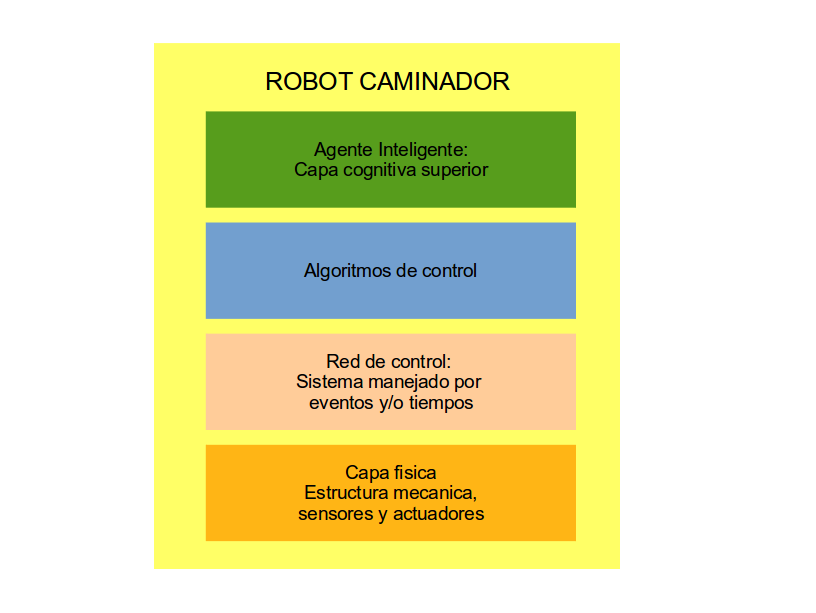
\includegraphics[height=7.0cm]{../images/objGen.png}
    \end{center}
  \end{frame}
}
\tagged{handout-tufte}{
  \begin{marginfigure}[-8.5cm]
    \centering
    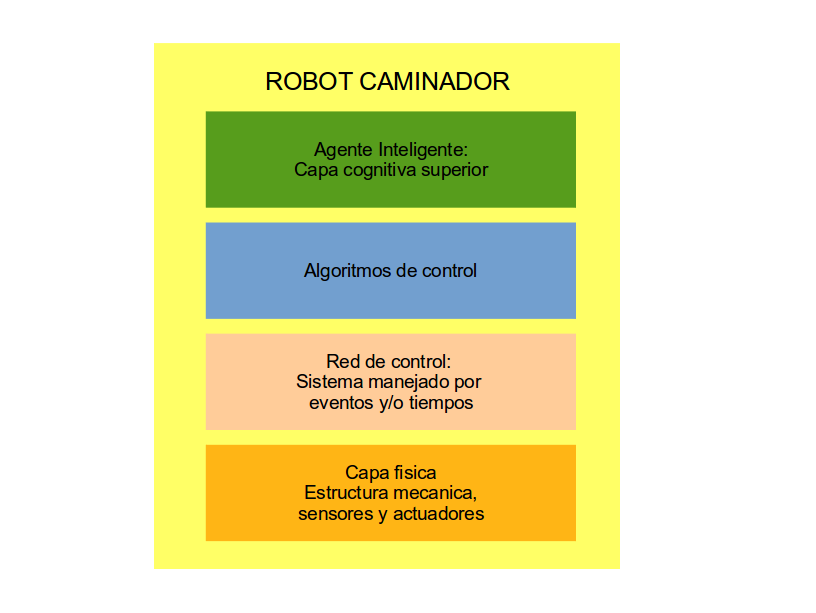
\includegraphics{../images/objGen.png}
    \caption{Objetivo General}
    \label{fig:objGen}
  \end{marginfigure}
}
\untagged{handout-tufte}{El principal objetivo de esta investigaci\'on se describe de forma global y gr\'afica en la Figura \ref{fig:objGen}, y es enunciado a continuaci\'on:\par}
\textbf{OG:} Dise\~nar y construir un \emph{\textbf{marco de experimentaci\'on}}\iftagged{handout-tufte}{%
  \sidenote[][-2.2cm]{\textbf{Marco de Experimentaci\'on:}
    {\scriptsize Es un aparato de conocimiento din\'amico con ejemplos construidos de plataformas b\'ipedas rob\'oticas que siguen los siguientes pasos:}
    \begin{enumerate}\tiny
    \item Selecci\'on de plataforma
    \item Dise\~no mecanico
    \item Dise\~no electronico 
    \item Sistema distribuido
    \item Capa de aplicaciones
    \end{enumerate}
  }
}{\footnote{compuesto por el dise\~no de una red de sensores-actuadores distribuida y un conjunto de dise\~no de eslanbones y articulaciones modulares para ser frabricados mediante prototipado r\'apido}} mediante el cual se pueda implementar\footnote{estudiar, proponer y/o comprobar} las hip\'otesis que solucionen los \emph{\textbf{problemas de locomoci\'on}}\iftagged{handout-tufte}{%
  \sidenote{\textbf{Problemas de la robotica b\'ipeda:}
    {\scriptsize Estan relacionados con el uso eficiente de la energ\'ia, la din\'amica pasiva de caminadores, presentes en:}
    \begin{enumerate}\tiny
    \item Estructuras mec\'anicas 
    \item Capa sensora y de actuaci\'on
    \item Control 
    \item Plan. y gen. de trayectorias 
    \item Capa de cognitiva
    \end{enumerate}
  }
}{\footnote{que permita la b\'usqueda de estructuras mecatr\'onicas eficientes energ\'eticamente, capaces de lograr la locomoci\'on requerida por las necesidades fundamentales de los robots caminadores}} de la rob\'otica subactuada y de caminadores\iftagged{handout-tufte}{ (Ver Figura. \ref{fig:objGen})}{}.\par
\untagged{handout-tufte}{
  \begin{figure}[!htb]
    \centering
    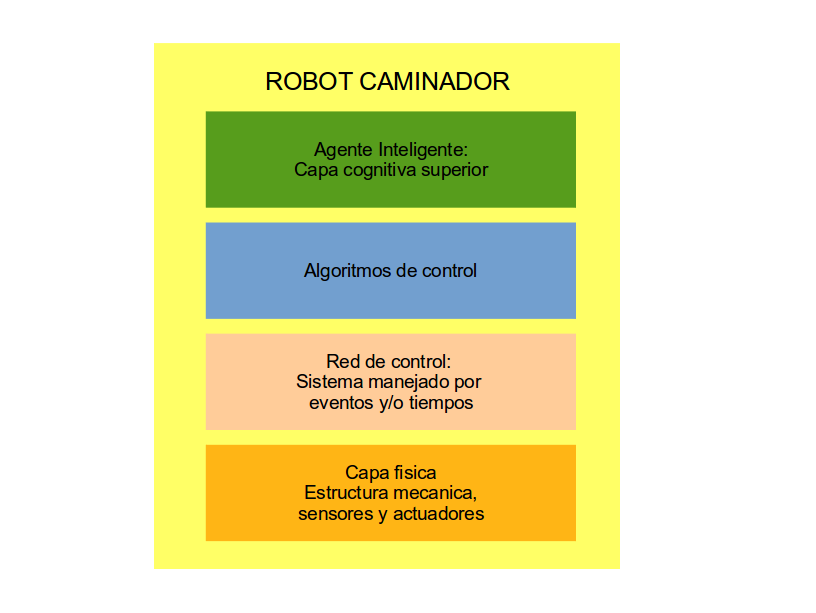
\includegraphics[scale=0.5]{../images/objGen.png}
    \caption{Objetivo General}
    \label{fig:objGen}
  \end{figure}
}

\mode<article|presentation>{%
  \iftagged{handout-tufte}%
  {\subsection[Especificos]{\textbf{Objetivos espec\'ificos}}}
  {\subsection[Especificos]{Objetivos especificos}}
}%
%\subsection[Especificos]{\iftagged{handout-tufte}{\textbf{Objetivos espec\'ificos}}{Objetivos espec\'ificos}}
\label{sec:objesp}
\mode<presentation>{
  \begin{frame}[label=def_objesp]
    \defObjespTime
    \frametitle{Qu\'e se requiere y qu\'e se obtiene para el Obj. Gen?}
    \framesubtitle{Algunos logros requeridos para el objetivo principal}
    \begin{center}
      \hyperlink{exp_capas<2>}{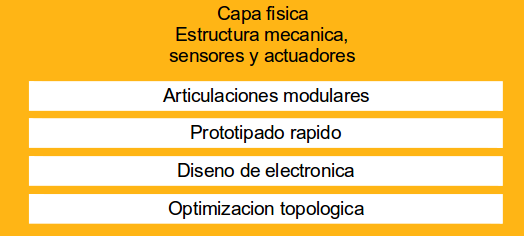
\includegraphics[height=2.0cm]{../images/objCapaFisica.png}}
      \hyperlink{exp_capas<3>}{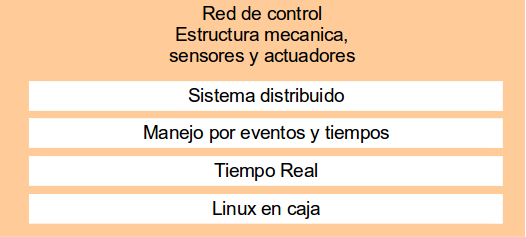
\includegraphics[height=2.0cm]{../images/objCapaRAS.png}}\\
      \hyperlink{exp_capas<4>}{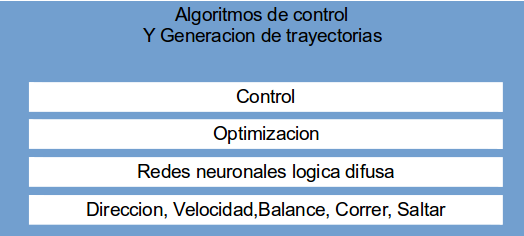
\includegraphics[height=2.0cm]{../images/objCapaControl.png}}
      \hyperlink{exp_capas<5>}{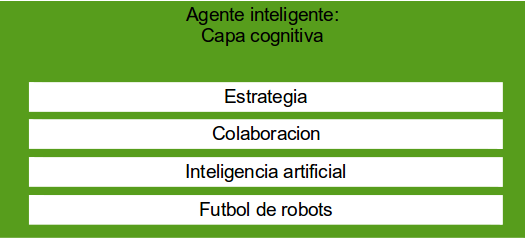
\includegraphics[height=2.0cm]{../images/objCapaCognitiva.png}}
    \end{center}
    \hyperlink{exp_capas}{\beamergotobutton{Explicaci\'on de Capas}}
  \end{frame}
}
\begin{enumerate}[\textbf{OE:} 1.]\tagged{handout-tufte}{\small}
\item Modelar, simular, analizar y sintetizar mecanismos subactuados que optimicen la energ\'ia para la locomoci\'on de caminar, saltar o correr.\untagged{handout-tufte}{\par}
\item Dise\~nar y construir una plataforma rob\'otica modular modular y para prototipado (ver Figura \ref{fig:objCapas} Capa Física), capaz de configurar cadenas cinem\'aticas  controladas y/o monitoreadas bajo el sistema distribuido\untagged{handout-tufte}{.\par}
\item Implementar un sistema distribuido de sensores y actuadores que funcione en tiempo-real  (ver Figura \ref{fig:objCapas} Capa de sensorial y de Actuaci\'on), bajo el principio de manejo por disparo-de-eventos y/o manejo por disparo-por-tiempos\untagged{handout-tufte}{\cite{Kimm2012}}.\par
\item Dise\~nar, simular e implementar diferentes controles de locomoci\'on (ver Figura \ref{fig:objCapas} Capa de control de locomoci\'on) inspirados en las nuevas tendencias de investigaci\'on de caminadores sobre plataformas rob\'oticas modulares construidas.\par
\item Dise\~nar, simular e implementar estrategias y actividades colaborativas usando una red de caminadores  (ver Figura \ref{fig:objCapas} Capa Cognitiva.).\par
\end{enumerate}
\iftagged{handout-tufte}{
  \begin{marginfigure}[-9.0cm]
    \centering
    %\parbox{11.6cm}{
      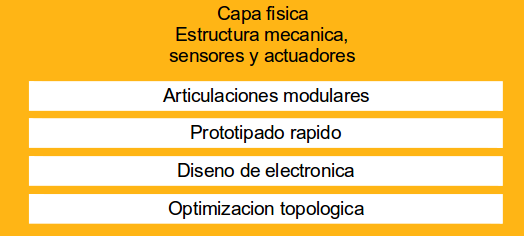
\includegraphics[width=5.0cm]{../images/objCapaFisica.png}\\
      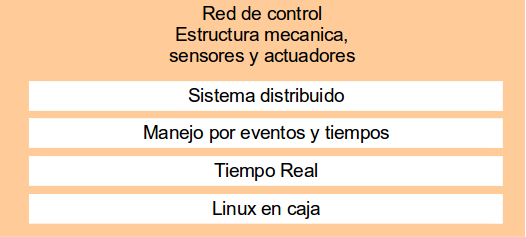
\includegraphics[width=5.0cm]{../images/objCapaRAS.png}\\
      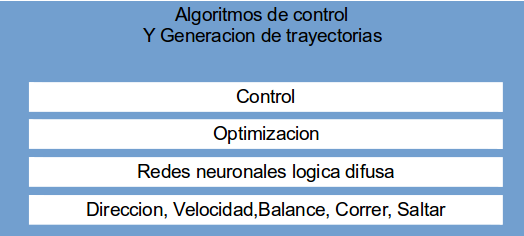
\includegraphics[width=5.0cm]{../images/objCapaControl.png}\\
      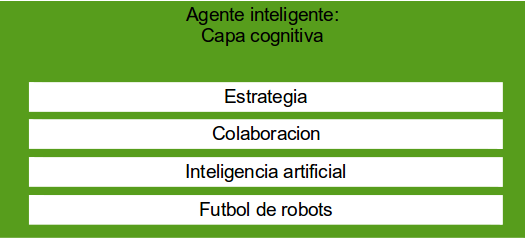
\includegraphics[width=5.0cm]{../images/objCapaCognitiva.png}
    %}\\
    \caption{Objetivos Específicos}
    \label{fig:objCapas}
  \end{marginfigure}
}{\begin{figure}[!htb]
    \centering
    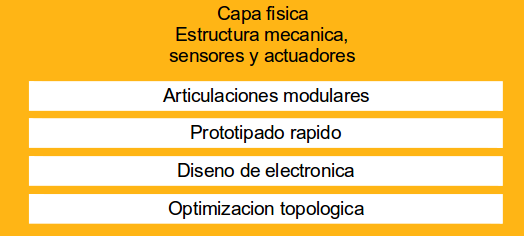
\includegraphics[scale=0.45]{../images/objCapaFisica.png}
    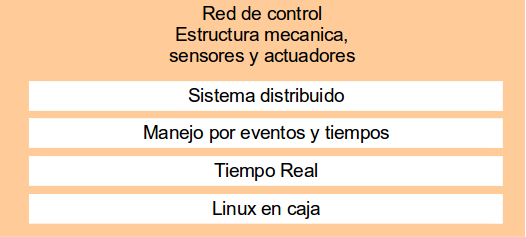
\includegraphics[scale=0.45]{../images/objCapaRAS.png}\\
    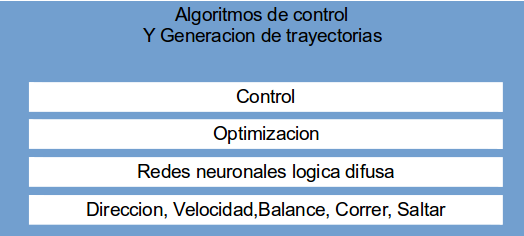
\includegraphics[scale=0.45]{../images/objCapaControl.png}
    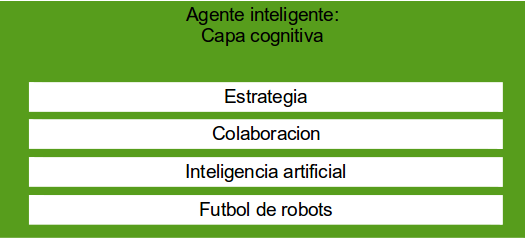
\includegraphics[scale=0.45]{../images/objCapaCognitiva.png}
    \caption{Objetivos Específicos}
    \label{fig:objCapas}
  \end{figure}
}
\mode<all>
\mode*
% \tagged{handout-tufte}{\vspace{-0.5cm}}
% \section[Estado del arte]{\iftagged{handout-tufte}{\textbf{\textcolor{blueun}{Estado del arte}}}{Estado del arte}}
\mode<article|presentation>{%
  \iftagged{handout-tufte}%
  {\section[Estado del arte]{\textbf{\textcolor{blueun}{Estado del arte}}}}%
  {\section[Estado del arte]{Estado del arte}}
}%
\label{sec:arte}
\mode<article>{%
  \tagged{handout-tufte}{
    % \subsection[Investigaci\'on actual]{\textbf{Algunas trabajos de investigaci\'on en la actualidad}}
    % \label{sec:algtra}
    A continuaci\'on el resumen de tendencias basada en la linea de tiempo del la Figura.\ref{fig:timelineH}. Adem\'as de lo anterior se muestra el estado actual del la Universidad Nacional en el tema (ver Figura.\ref{fig:timelineH}).
    \vspace{-0.3cm}
    \subsection[Resumen]{\textbf{Resumen de tendencias}}
    \label{sec:resten}
    \vspace{-1.0cm}
    \begin{figure}%[!htb]
      \centering
      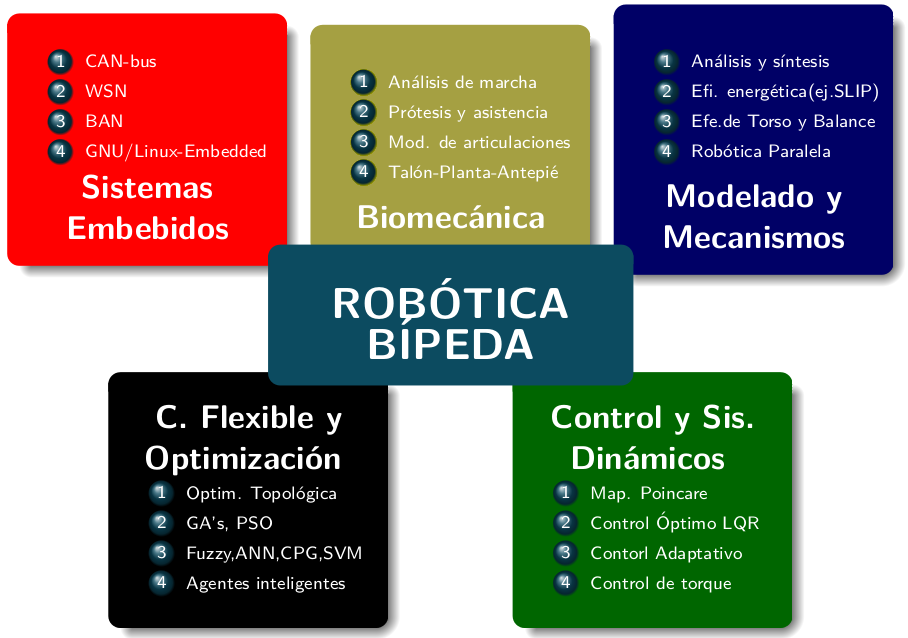
\includegraphics{../images/Resumen.png}
      \caption{Resumen de las tendencias de investigaci\'on}
      \label{fig:resTendencias}
    \end{figure}
    \begin{marginfigure}[-10.0cm]%[!h]
      \centering
      \includegraphics{../images/TimeLine05.png}
      \caption{L\'inea de tiempo: Tendencias de distingas universidaes destacadas en Caminadores}
      \label{fig:timelineH}
    \end{marginfigure}
    \begin{marginfigure}[-2.0cm]
      \centering
      % \includegraphics[height=4.5cm]{../images/UNROCA_3.png}
      \includegraphics[height=4.5cm]{../images/UNROCA_5.png}
      \includegraphics[height=4.5cm]{../images/UNROCA_6.png}
      \caption{Proyecto UNROCA de la UN}
      \label{fig:rocaUN}
    \end{marginfigure}
  }
}
\mode<presentation>{
  \begin{frame}[label=arte]
    \transduration{2}
    \frametitle{Cu\'al es el estado actual de la Caminata B\'ipeda?}
    \framesubtitle{Antecedentes y tendencias mundiales de investigaci\'on}
    \begin{center}
      \LARGE \textbf{\textcolor{blueun}{Estado del Arte}}
    \end{center}      
  \end{frame}
  \subsection[Investigaci\'on actual]{Algunas trabajos de investigaci\'on en la actualidad }
  \label{sec:algtra}
  \begin{frame}[label=timeline]
    \transduration{10}
    \frametitle{Breve historia de la rob\'otica b\'ipeda}
    \framesubtitle{Para entrar en contexto}
    \includegraphics[height=7.5cm,width=10.0cm]{../images/TimeLine05.png}
  \end{frame}
  \begin{frame}[label=tendencias]
    \transduration<1->{3}
    \frametitle{Trabajos relevantes de los \'ultimos 8 a\~nos}
    \framesubtitle{Tendencias mundiales en investigaci\'on}
    \begin{columns}[T]
      \begin{column}{2.0cm}
        \setbeamercovered{transparent}
        \uncover<2>{\includegraphics[height=7.5cm]{../images/TimeLineTendencias01.png}}
      \end{column}
      \begin{column}{5.0cm}
        \only<1>{
          \begin{center}
            \textbf{\textcolor{blueun}{Universidad de Waseda}}
            \begin{center}
              \includegraphics[height=1.5cm]{../images/WasedaLogo.png}\\
            \end{center}
            \hspace{1.5cm}\includegraphics[height=3.8cm]{../images/WasedaTendencias.png}
          \end{center}
        }
        \only<2>{
          \begin{center}
            \textbf{\textcolor{blueun}{Honda Research Institute\\\& IHMC}}
            \begin{center}
              \includegraphics[height=0.7cm]{../images/HondaLogo.png}\quad
              \includegraphics[height=0.7cm]{../images/IHMCLogo.png}
            \end{center}
            \hspace{1.8cm}\includegraphics[height=4.0cm]{../images/HondaTendencias.png}            
          \end{center}
        }
        \only<3>{
          \begin{center}
            \textbf{\textcolor{blueun}{Aldebaran Robotics}}
            \begin{center}
              \includegraphics[height=1.0cm]{../images/AldebaranLogo.png}\\
            \end{center}
            \vspace{0.5cm}\hspace{0.3cm}\includegraphics[height=4.0cm]{../images/AldebaranTendencias.png}            
          \end{center}
        }
        \only<4>{
          \begin{center}
            \textbf{\textcolor{blueun}{MIT\\Robot Locomotion Group}}\\
            \begin{center}
              \includegraphics[height=1.0cm]{../images/MITLogo.png}
            \end{center}
            \vspace{0.5cm}\hspace{1.5cm}\includegraphics[height=3.0cm]{../images/MITTendencias.png}            
          \end{center}
        }
        \only<5>{
          \begin{center}
            \textbf{\textcolor{blueun}{ETH-BIRLab}}\\
            \begin{center}
              \includegraphics[height=1.0cm]{../images/ETHLogo.png}
            \end{center}
          \vspace{0.5cm}\hspace{1.5cm}\includegraphics[height=4.0cm]{../images/ETHTendencias.png}
          \end{center}
        }
        \only<6>{
          \begin{center}
            \textbf{\textcolor{blueun}{CMU - Biorobotics and \\ CU - Locomotion Labs}}
            \begin{center}
              \includegraphics[height=0.7cm]{../images/CMULogo.png}\\
              \includegraphics[height=0.7cm]{../images/CornellULogo.png}
            \end{center}
            \vspace{0.1cm}\hspace{1.5cm}\includegraphics[height=3.5cm]{../images/CMUCornellTendencias.png}
          \end{center}
        }
        \only<7>{
          \begin{center}
            \textbf{\textcolor{blueun}{Delft University-DBL Lab}}\\
            \begin{center}
              \includegraphics[height=1.0cm]{../images/DelftLogo.png}\\
            \end{center}
            \vspace{0.1cm}\hspace{2.5cm}\includegraphics[height=4.0cm]{../images/DelftTendencias.png}
          \end{center}
        }
        \only<8>{
          \begin{center}
            \textbf{\textcolor{blueun}{Gottingen University}}
            \begin{center}
              \includegraphics[height=1.5cm]{../images/GottingenULogo.png}
            \end{center}
            \vspace{0.1cm}\hspace{2.0cm}\includegraphics[height=3.5cm]{../images/GottingenUTendencias.png}
          \end{center}
        }
        \only<9>{
          \begin{center}
            \textbf{\textcolor{blueun}{CNRS}}
            \begin{center}
              \includegraphics[height=2.0cm]{../images/CNRSLogo.png}\\
            \end{center}
            \vspace{0.1cm}\hspace{2.0cm}\includegraphics[height=3.5cm]{../images/CNRSTendencias.png}
          \end{center}
        }
        \only<10>{
          \begin{center}
            \textbf{\textcolor{blueun}{DLR-biped}}
            \begin{center}
              \includegraphics[height=1.0cm]{../images/DLRLogo.png}\\
            \end{center}
            \vspace{0.1cm}\hspace{1.0cm}\includegraphics[height=4.0cm]{../images/DLRTendencias.png}
          \end{center}
        }
      \end{column}
      \begin{column}{3.5cm}
        \only<1>{
          \begin{center}
            \vspace{1.3cm}
            \textbf{\textcolor{blueun}{Tendencias}}
            \begin{itemize}\scriptsize
            \item Rob\'otica paralela
            \end{itemize}
            %\includegraphics[height=1.0cm]{../images/WasedaTendencias01.png}            
          \end{center}
        }
        \only<2>{
          \begin{center}
            \vspace{1.3cm}
            \textbf{\textcolor{blueun}{Tendencias}}
            \begin{itemize}\scriptsize
            \item Control
            \item Efectos del Torso
            \end{itemize}
          \end{center}
        }
        \only<3>{
          \begin{center}
            \vspace{1.3cm}
            \textbf{\textcolor{blueun}{Tendencias}}
            \begin{itemize}\scriptsize
            \item CPG, ANN
            \item AI, Aprendizaje
            \end{itemize}
          \end{center}
        }
        \only<4>{
          \begin{center}
            \vspace{1.3cm}
            \textbf{\textcolor{blueun}{Tendencias}}
            \begin{itemize}\scriptsize
            \item Control:{\tiny LQR-trees, SVM}
            \item Rob\'otica subactuada
            \end{itemize}
          \end{center}
        }
        \only<5>{
          \begin{center}
            \vspace{1.3cm}
            \textbf{\textcolor{blueun}{Tendencias}}
            \begin{itemize}\scriptsize
            \item Bajo costo
            \item CPG, SVM
            \item BAN
            \end{itemize}
          \end{center}
        }
        \only<6>{
          \begin{center}
            \vspace{1.3cm}
            \textbf{\textcolor{blueun}{Tendencias}}
            \begin{itemize}\scriptsize
            \item Balanceo, torso, SLIP
            \item Talon y tobillo
            \item Modelos Masa-resorte
            \end{itemize}
          \end{center}
        }
        \only<7>{
          \begin{center}
            \vspace{1.3cm}
            \textbf{\textcolor{blueun}{Tendencias}}
            \begin{itemize}\scriptsize
            \item Running robot
            \item Air Muscles and DC motors
            \item Balance
            \end{itemize}
          \end{center}
        }
        \only<8>{
          \begin{center}
            \vspace{1.3cm}
            \textbf{\textcolor{blueun}{Tendencias}}
            \begin{itemize}\scriptsize
            \item Aprendizaje de m\'aquina
            \item Control adaptativo
            \item Running Mode
            \end{itemize}
          \end{center}
        }
        \only<9>{
          \begin{center}
            \vspace{1.3cm}
            \textbf{\textcolor{blueun}{Tendencias}}
            \begin{itemize}\scriptsize
            \item Control y trayectoria
            \item Running Mode
            \end{itemize}
          \end{center}
        }
        \only<10>{
          \begin{center}
            \vspace{1.3cm}
            \textbf{\textcolor{blueun}{Tendencias}}
            \begin{itemize}\scriptsize
            \item Capture Points
            \item Control de torque de cuerpo completo
            \item Agarre de cuerpo completo
            \end{itemize}
          \end{center}
        }
      \end{column}
    \end{columns}
  \end{frame}
}
\untagged{handout-tufte}{
  Revisando la amplia literatura encontrada sobre \emph{la locomoci\'on}, la mayor inquietud citada viene de la Rob\'otica\cite{Xiang2010,Mattar2013} y la Biomec\'anica\cite{Xiang2010,Mattar2013}, \'areas que muestran su interés en replicar las estructuras y/o las funcionalidades de movilidad de diferentes seres vivos\cite{Xu2013,Chiang2013} o como muchos autores\cite{Xu2013} y congresos\cite{RB2009} hacen referencia a \emph{biom\'imesis}. Estas necesidades van desde solo comprobar las leyes f\'isicas sobre un sistema mecatr\'onico\cite{Barker2010,Lens2011} hasta dise\~nar m\'aquinas robotizadas que sirvan al hombre en ambientes de riesgo donde \'este no deber\'ia encontrarse\cite{Seifried2014,Wu2013a}, o desde solo entender la marcha humana para proponer una terap\'ia sobre alg\'un m\'usculo lesionado\cite{Kang2013} hasta el remplazo de una extremidad que mejore la calidad de vida de una persona v\'ictima de alg\'un accidente\cite{Roa2006,Wu2013a}.\par
  Dentro de la locomoci\'on b\'ipeda se diferencia dos formas generales del modo de andar: una bajo el r\'egimen de caminata y otra bajo el r\'egimen de correr, trotar o galopar\cite{Geyer2006}. La manera de distinguir estos modos viene dada por las distintas fase que definen un ciclo de andar, la diferencia entre caminar y trotar, ser\'a que durante la caminata habr\'an fases con doble contacto con el piso, mientras que en el r\'egimen de trotar o correr no existirá fases con doble contacto\cite{Geyer2006}, adem\'as en el regim\'en de correr existe una fase en la que no ocurre ningún contacto, fase que se encuentra con el nombre de vuelo.\par
  Una de las posibles clasificaciones que se pude hacer en caminadores es seg\'un su tipo de balance durante la caminata, este balance puede ser est\'atico o din\'amico\cite{Braunl2008}. Las mayores inquietudes y retos al d\'ia de hoy se encuentran en el balance din\'amico, pues este tipo de balance se acerca m\'as a una caminata \'optima y natural, como la que han logrado los seres humanos durante toda su evoluci\'on.\par
  Otra clasificaci\'on podr\'ia ser los modelos físico, que se han utilizado para describir la caminata\cite{Xiang2010}: 1) modelos de p\'endulo invertido, 2) din\'amica pasiva de la caminata y 3) ZMP punto de momento cero. Una caracter\'istica de los tres modelos f\'isico citados anteriormente, es que sus movimientos son generados en tiempo real\cite{Xiang2010}. En el caso de la din\'amica pasiva de la caminata, recientes tendencias en b\'usqueda de dise\~nos naturales tanto en las estructuras mec\'anicas como en los esquemas de control buscan mejorar los problemas energ\'eticos que resultaron de los mejores avances que se han obtenido en el tema gracias al concepto del ZMP\cite{Xiang2010}.\par
  Aunque la caminata pasiva lleva en estudio m\'as de 25 a\~nos, tuvo un momento de oscuridad cuando el ZMP, el cual lleva m\'as de 40 a\~nos, logr\'o resultados tecnol\'ogicos en los a\~nos ochenta\cite{Vukobratovic2004}. Desde hace 25 a\~nos se retomo nuevamente el estudio de la caminata pasiva ya no solo como ejemplo acad\'emico\cite{McGeer1990a}, dando nuevos caminos en el control y acerc\'andose a la soluci\'on desde el punto de vista de la optimizaci\'on de la energ\'ia\cite{Goswami1996}, proponiendo as\'i a la caminata activa la generaci\'on \'optima de trayectorias\cite{Gregg2010}.\par
  Los modelo mec\'anicos bio-inspirados se encuentran de dos clases\cite{Xiang2010}. El primero que toma el sistema \'oseo para luego proponer unos actuadores distintos a los músculos\cite{Wang2012} y el segundo que analiza adem\'as del sistema \'oseo, el sistema muscular para tomar los m\'usculos del cuerpo humano como los actuadores del sistema\cite{Kang2013,Roa2006}. Los modelos matem\'aticos de estos modelos bio-inspirados est\'an basados en la din\'amica multicuerpo\cite{Xiang2010}, donde cabe resaltar que los modelos m\'usculo-esquel\'eticos incrementan la carga computacional por el gran n\'umero de grados de libertad\cite{Xiang2010}, mientras que los modelos basados \'unicamente en el sistema oseo son f\'aciles de simplificar y en la mayor\'ia de los casos tan solo se tiene en cuenta las longitudes de las extremidades analizadas reduciendo también un importante n\'umero de grados de libertad\cite{McGeer1990a}. Cabe resaltar de diferentes herramientas y formalismos son empleadas en la literatura para la generaci\'on de modelos, en donde se encuentran: Newton-Euler, Euler-Lagrange, Hamilton, Kane, \'algebras especiales para entender el espacio tridimensional como los Screws y los cuaterniones o el método de Denavit-Hartenverg y finalmente la conservaci\'on del momento angular para representar las colisiones de los sistemas.\par
  Dentro del problema de la din\'amica multicuerpo, se enfrentan dos pilares, 1) la din\'amica inversa, donde las trayectorias se conocen en un comienzo o se pueden tomar arbitrarias para luego encontrar las cargas requeridas por los actuadores y 2) la din\'amica directa en donde se conocen las cargas en los actuadores, y resolviendo un sistema de ecuaciones diferenciales con condiciones iniciales de segundo orden se puede encontrar la evoluci\'on temporal de las articulaciones en el espacio.\par
  Una vez se logra un modelo f\'isico del caminador, surgen los problemas de generaci\'on de las trayectorias. La generaci\'on de trayectorias es un problema abierto que se aborda con muchas t\'ecnicas y seg\'un los objetivos de la investigaci\'on\cite{Kherici2014,Mahmoodabadi2014}. Una clasificaci\'on dada por\cite{Xiang2010}, divide la generaci\'on de trayectorias en m\'etodos basados en optimizaci\'on y m\'etodos basados en control. Ambos son lo suficientemente costos para ser implementados en tiempo real sin exagerar los recursos de c\'omputo\cite{Mahmoodabadi2014}. Adem\'as de esto es com\'un emplear los m\'etodos de optimizaci\'on y control en conjunto para encontrar la soluci\'on.\par
  Las dificultades presentes en la generaci\'on de trayectorias tienen 1) la complejidad computacional de la programaci\'on no-lineal adem\'as de una optimizaci\'on multiobjetivo, en la que se pueden encontrar restricciones de diferentes clases\cite{Mahmoodabadi2014}, 2) los modelos h\'ibridos presentes en los modelos de mec\'anica multicuerpo introducen discontinuidades en las funciones objetivo, lo que propone que los m\'etodos de b\'usqueda basados gradiente sean descartados\cite{Xiang2010}, tambi\'en se proponer mediciones del rendimiento de la marcha que eviten dichas discontinuidades para usar los m\'etodos de b\'usqueda basados en gradiente\cite{Xiang2010}.\par
  Dependiendo como se aborde el problema de la din\'amica, inverso o directo, es posible que la generaci\'on de las trayectorias implique, la soluci\'on de las ecuaciones diferenciales, este es el caso de la d\'inamica directa en el que se proponen las cargas sobre el sistema pero se desconocen las trayectorias, es ac\'a cuando la variable de dise\~no en este caso las cargas, se deben buscar la mejor evoluci\'on de cargas en el tiempo, que satisfaga las condiciones de dise\~no.\par
}
\untagged{handout-tufte}{\subsection[Estado del arte UN]{Estado del arte en la Universidad Nacional de Colombia}
\label{sec:estadoUN}}
\tagged{handout-tufte}{
  % \label{sec:resten}
  % \begin{figure}%[!htb]
  %   \centering
  %   \includegraphics{../images/Resumen.png}
  %   \caption{L\'inea de tiempo}
  %   \label{fig:timelineH}
  % \end{figure}
  % \begin{marginfigure}[0.0cm]
  %   \centering
  %   \includegraphics[height=5cm]{../images/UNROCA_5.png}
  %   \includegraphics[height=5cm]{../images/UNROCA_6.png}
  %   \caption{Proyecto UNROCA de la UN}
  %   \label{fig:rocaUN}
  % \end{marginfigure}
}
\mode<presentation>{
  \begin{frame}[label=tendenciasUN]
    \transduration<1->{2}
    \frametitle{Cual es la actualidad y antecedentes en la UN?}
    \framesubtitle{Robotica b\'ipeda y temas afines desarrollados en la UN}
    \begin{columns}[T]
      \begin{column}{6cm}
        \setbeamercovered{transparent}
        Descripci\'on serie UNROCA:
        \begin{enumerate}\scriptsize
        \item<2-> Modelo PWD con rodillas
        \item<3-> Ciclos L\'imite
        \item<4-> Bifurcaciones y caos
        \item<5-> Metodolog\'ia de dise\~no
        \item<6-> UNROCA-I
        \item<7-> UNROCA-II
        \item<8-> UNROCA-III
        \end{enumerate}
        \visible<9->{\uncover<9->{
        Temas relacionados:
        \begin{enumerate}\scriptsize
        \item<10-> Rob\'otica subactuada
        \item<11-> Caminata animal b\'ipeda
        \end{enumerate}}}
      \end{column}
      \begin{column}{4cm}
        \vspace{-0.5cm}
        \only<1>{
          \begin{center}
            \includegraphics[height=7cm]{../images/UNROCA.png}
          \end{center}
        }
        \only<2>{
          \begin{center}
            \includegraphics[height=7cm]{../images/UNROCA_0.png}
          \end{center}
        }
        \only<3>{
          \begin{center}
            \includegraphics[height=7cm]{../images/UNROCA_1.png}
          \end{center}
        }
        \only<4>{
          \begin{center}
            \includegraphics[height=7cm]{../images/UNROCA_2.png}
          \end{center}
        }
        \only<5>{
          \begin{center}
            \includegraphics[height=7cm]{../images/UNROCA_3.png}
          \end{center}
        }
        \only<6>{
          \begin{center}
            \includegraphics[height=7cm]{../images/UNROCA_4.png}
          \end{center}
        }
        \only<7>{
          \begin{center}
            \includegraphics[height=7cm]{../images/UNROCA_5.png}
          \end{center}
        }
        \only<8>{
          \begin{center}
            \includegraphics[height=7cm]{../images/UNROCA_6.png}
          \end{center}
        }
        \only<9-10>{
          \begin{center}
            \includegraphics[height=7cm]{../images/UNRSubactuada.png}
          \end{center}
        }
        \only<11>{
          \begin{center}
            \includegraphics[height=7cm]{../images/UNACaminata.png}
          \end{center}
        }
      \end{column}
    \end{columns}
  \end{frame}
  \subsection[Resumen]{Resumen de tendencias }
  \label{sec:resten}
  \begin{frame}[label=resumen]
    \transduration<1-7>{0.8}
    \frametitle{Hacia una framework de rob\'otica b\'ipeda}
    \framesubtitle{Resumen de tendencias por \'area en Rob\'otica B\'ipeda}
    \begin{center}
      \only<1-7>{
        \vspace{-2.2cm}
        \begin{columns}[c]
          \begin{column}{3cm}
            \only<1,3-6>{\setbeamercolor{postit}{fg=white,bg=red!40!black}}
            \only<2,7>{\setbeamercolor{postit}{fg=white,bg=red}}
            \begin{beamercolorbox}[sep=0.5em,wd=3cm,rounded=true,center,shadow=true]{postit}
              \begin{enumerate}\tiny
              \item CAN-bus
              \item WSN
              \item BAN
              \item GNU/Linux-Embedded
              \end{enumerate}
              \textbf{Sistemas Embebidos}
            \end{beamercolorbox}
          \end{column}
          \begin{column}{3cm}
            \only<1-2,4-6>{\setbeamercolor{postit}{fg=white,bg=yellow!60!black}}
            \only<3,7>{\setbeamercolor{postit}{fg=white,bg=yellow}}
            \begin{beamercolorbox}[sep=0.5em,wd=3cm,rounded=true,center,shadow=true]{postit}
              \begin{enumerate}\tiny
              \item An\'alisis de marcha
              \item Pr\'otesis y asistencia
              \item Mod. de articulaciones
              \item Tal\'on-Planta-Antepi\'e
              \end{enumerate}
              \textbf{Biomec\'anica}
            \end{beamercolorbox}
          \end{column}
          \begin{column}{3cm}
            \only<1-3,5-6>{\setbeamercolor{postit}{fg=white,bg=blue!40!black}}
            \only<4,7>{\setbeamercolor{postit}{fg=white,bg=blue}}
            \begin{beamercolorbox}[sep=0.5em,wd=3cm,rounded=true,center,shadow=true]{postit}
              \begin{enumerate}\tiny
              \item An\'alisis y s\'intesis
              \item Efi. energ\'etica(ej.SLIP)
              \item Efe.de Torso y Balance
              \item Rob\'otica Paralela
              \end{enumerate}
              \textbf{Modelado y Mecanismos}
            \end{beamercolorbox}
          \end{column}
        \end{columns}
        \vspace{1.0cm}
        \begin{columns}[c]
          \begin{column}{3cm}
            \only<1-4,6>{\setbeamercolor{postit}{fg=white,bg=black}}
            \only<5,7>{\setbeamercolor{postit}{fg=white,bg=white!50!black}}
            \begin{beamercolorbox}[sep=0.5em,wd=3cm,rounded=true,center,shadow=true]{postit}
              \textbf{C. Flexible y Optimizaci\'on}
              \begin{enumerate}\tiny
              \item Optim. Topol\'ogica
              \item GA's, PSO
              \item Fuzzy,ANN,CPG,SVM
              \item Agentes inteligentes
              \end{enumerate}
            \end{beamercolorbox}
          \end{column}
          \begin{column}{3cm}
            \only<1-5>{\setbeamercolor{postit}{fg=white,bg=green!40!black}}
            \only<6,7>{\setbeamercolor{postit}{fg=white,bg=green}}
            \begin{beamercolorbox}[sep=0.5em,wd=3cm,rounded=true,center,shadow=true]{postit}
              \textbf{Control y Sis. Din\'amicos}
              \begin{enumerate}\tiny
              \item Map. Poincare
              \item Control \'Optimo LQR
              \item Contorl Adaptativo
              \item Control de torque
              \end{enumerate}
            \end{beamercolorbox}
          \end{column}
        \end{columns}
        \vspace{-4.6cm}
        \hspace{-0.25cm}
        \setbeamercolor{postit}{fg=white,bg=blueun}
        \begin{beamercolorbox}[sep=0.5em,wd=4.0cm,rounded=true,center]{postit}
          \textbf{\Large\textcolor{white}{ROB\'OTICA B\'IPEDA}}
        \end{beamercolorbox}
      }
    \end{center}
  \end{frame}
}
\untagged{handout-tufte}{
El departamento de Ingenier\'ia Mec\'anica y Mecatr\'onica hacia 2003, bajo los grupos de investigaci\'on de Biomec\'anica y Robots M\'oviles, construye tres modelos de caminadores, en donde las patrones de marcha son generados por el an\'alisis y simulaci\'on de caminadores pasivos y posteriormente las trayectorias de las articulaciones son reproducidas por los caminadores activos construidos. Adicionalmente se propone una metodolog\'ia de dise\~no\cite{Heredia2007}.\par
El modelo de tres eslabones y cuatro masas puntales cl\'asico estudiado antes por\cite{McGeer1990a}, se obtienen distintas trayectorias de los \'angulos de las articulaciones para diferentes velocidades de marcha que son directamente relacionadas con las pendientes de inclinaci\'on del piso\cite{M2005}, es importante mencionar que se incluye un an\'alisis adimensional de parámetros y un an\'alisis de las propiedades ca\'oticas del caminador bípedo analizado\cite{M2005a}. Los datos obtenidos en la fase anterior, son convertidos a los requeridos por la construcci\'on f\'isica implementada.\par
A continuaci\'on se muestran los tres robot UNROCA generados en el departamento Figura.\ref{fig:unroca}, los dos primeros intentos mostraban la reproducci\'on de las trayectorias generadas en la primera fase, pero usaban soportes estructurales para alcanzar la estabilidad. En el tercer intento el robot aseguro su estabilidad con el uso de una masa oscilante a la altura de la cadera, se incorporan granes pies para la estabilidad est\'atica. Bajo el r\'egimen de marcha la estabilidad es asegurada en acci\'on del contrapeso oscilante y el criterio de ZMP de la trayectoria previamente calculada. La trayectoria es seguida usando controles PD y utilizando servomotores. Por cada par de servos es utilizado un microcontrolador m\'as un microcontrolador central\cite{M2005}.
\begin{figure}[!hbt]
  \centering
  \includegraphics[scale=0.4]{../images/unroca.png}
  \caption{Robots serie UNROCA. [Tomado de \cite{M2005}]}
  \label{fig:unroca}
\end{figure}
}
\mode<article>{
\untagged{handout-tufte}%{\subsection[Resumen]{\textbf{Resumen de tendencias}}
  % \label{sec:resten}
  % \begin{figure}%[!htb]
  %   \centering
  %   \includegraphics{../images/Resumen.png}
  %   \caption{L\'inea de tiempo}
  %   \label{fig:timelineH}
  % \end{figure}
  % \begin{marginfigure}[0.0cm]
  %   \centering
  %   \includegraphics[height=5cm]{../images/UNROCA_5.png}
  %   \includegraphics[height=5cm]{../images/UNROCA_6.png}
  %   \caption{Proyecto UNROCA de la UN}
  %   \label{fig:rocaUN}
  % \end{marginfigure}
  % }
{
  \subsection[Investigaci\'on actual]{Algunas trabajos de investigaci\'on en la actualidad }
  \label{sec:algtra}

  \subsubsection[Gen. Tray. y Control]{Generaci\'on de trayectorias y control}
  \label{sec:gentray}
  Simulaci\'on de un robot b\'ipedo empleando una m\'etodo evolutivo. 10 DOF y 7 eslabones, el m\'etodo PSO (Particle swarm optimization) asegura la estabilidad usando como restricci\'on el centro de masa CoM del pol\'igono de soporte\cite{Kherici2014}.\par
  Se compara varios m\'etodos de optimizaci\'on multiobjetivo NSGAII, Sigma method, MOGA con el m\'etodo MOPSO. El m\'etodo es utilizado para sintonizar un controlador "robust sliding tracking". En el proceso se reduce una b\'usqueda heur\'istica de parámetros por ensayo-error, a una b\'usqueda \'optima seg\'un criterios de dise\'~no. Un operador de turbulencia es utilizado para evadir \'optimos locales\cite{Mahmoodabadi2014}.\par
  Se proponen trayectorias \'optimas y din\'amicamente estables para subir y bajar escaleras basadas en el movimiento humano. Siete caracter\'isticas son resaltadas. Un algoritmo gen\'etico de c\'odigo real es utilizado para optimizar la marcha del robot y mejorar el consumo de energ\'ia y fortalecer la estabilidad. Simulaciones sobre configuraciones de 12-DOF son simuladas, basadas en las capturadas del movimiento humano durante el ascenso y el descenso de escaleras\cite{Lim2014}.\par
  Se emplea un control (0-flat normal form) en una plataforma b\'ipeda de 7-DOF. Los resultados obtenidos muestran el buen desempe\~no de este m\'etodo para proponer leyes de control en sistemas altamente no-lineales. Adicional se propone una estrategia de dise\~no para controladores en robots caminadores\cite{Bououden2014}.\par
  Se plantea un control compensado para evitar que perturbaciones externas, saquen de control el sistema. El sistema de aprendizaje mediante m\'aquinas de soporte vectorial difuso. Los resultados son comparados con otros m\'etodos inteligentes y se muestra su superioridad, mostrando una mayor sensibilidad y aumentando los rangos de estabilidad. En las fases de SSP y DSP se introducen conjunto de pertenencia de  triangulares y Gauss que permiten formular propiedades temporales de las marchas de robots con perturbaciones externas\cite{Wang2013}.\par
  Usando el robot ePaddle, dise\~nado para actuar en medios terrestres, acu\'aticos y terrenos anfibios. Se estudia la marcha en modo carrera caminata. Simulaciones subiendo escaleras y siguiendo trayectorias circulares, muestran la estabilidad y eficiencia encontrada\cite{Sun2013}.\par
  Generaci\'on en tiempo real de trayectorias para un robot de siete eslabones planar\cite{Farzaneh2014}.\par

  \subsubsection[Bioinspiardos y mecanismos]{Biomec\'anica, Caminata,  Modelado y S\'intesis de mecanismos}
  \label{sec:ascapa}
  Un arreglo de sensores de fuerza flexible (FFSA) es construido para caracterizar el contacto del pie con terrenos irregulares, para determinar el área efectiva de contacto (ECA). Esta área es importante para mantener el balance dinámico y por lo tanto es utilizado en un esquema adicional de control para caminar sobre terrenos irregulares\cite{Wu2013}.\par
  Una rodilla basada en mecanismos de cuatro barras es investigada en el desempe\~no de robots bípedos. Es comparada con la articulaci\'on tradicional rotacional de los robots. Concluyendo que aunque para bajas velocidades la articulaci\'on rotacional es mejor, en altas velocidades el mecanismo de cuatro barras muestra un mejor desempe\~no. El mecanismo de cuatro barras es optimizado siguiendo los ciclos de marcha óptimos\cite{Aoustin2013}.\par
  Se dise\~na una rodilla (mediante optimizaci\'on perimétrica) basada en rodadura natural de la rodilla, se obtiene un mejoramiento en el consumo energético de los actuadores comparados con las rodillas de rotación tradicional\cite{Hobon2014}.\par
  Modelado del efecto del contacto de rodadura de la planta del pie en la dinámica de caminar. El contacto es descrito por las longitudes del retropie, mediopie y antepie. Los parámetros anteriores son relacionado con los principales descriptores de marcha como la velocidad media , el periodo de paso en ángulo de entrepierna y la longitud de paso, así como la energía mecánica. Estas relaciones resultan útiles para el dise\~no de prótesis y la estabilidad del sistema\cite{Mahmoodi2013}.\par
  Un nuevo dise\~no m\'as parecido a las características humanas en cuanto a la rodilla, el contacto de la planta del pie, inspirados en la forma del esqueleto humano, especialmente la pelvis. Las ventajas de la pelvis se ven reflejadas en el manejo del centro de gravedad de la parte superior del cuerpo humano. Un mejor modelo del pie conlleva a modelo de péndulo invertido durante sus fases\cite{Chiang2013}.\par
  Basados en el modelo de la din\'amica de la caminata pasiva, específicamente la marcha del compás, la cual exhibe propiedades de caos. Se linealiza el modelo alrededor de un ciclo limite híbrido. Usando los mapas de Poincar\'e, es dise\~na un control por realimentaci\'on de estados, para convertir el sistema pasivo en activo\cite{Gritli2013}.\par
  Se realiza el dise\~no de la lagartija Jesucristo, basado en un mecanismos Watt-I y los grupos de Assur. Se utiliza un algoritmo de control CPG(Central Pattern Generator) del sistema neural, para el balance y el ajusta de la marcha \cite{Xu2013}.\par
  Análisis del modelo dinámico, estabilidad y consumo de energ\'ia eficiente de un robot con seis extremidades\cite{Roy2013}.\par
}
}
\mode<all>
%\mode*
\section[Def. Problema]{Definici\'on del problema}
\label{sec:problema}

\mode<presentation>{
  \begin{frame}
    \transduration{1}
    \frametitle{Cu\'al es el problema?}
    \framesubtitle{Generaci\'on de rob\'otica b\'ipeda y soluci\'on a sus problemas}
    \begin{center}
      \LARGE \textbf{\textcolor{blueun}{Definici\'on del problema}}
    \end{center}      
  \end{frame}
}
\subsection[Identificaci\'on]{Identificaci\'on}
\mode<presentation>{
  \begin{frame}
    \transduration<1->{1}
    \frametitle{Qu\'e pas\'o?}
    \framesubtitle{Causas del receso en al investigaci\'on}
    \begin{center}
      \only<1>{\includegraphics[width=10.5cm]{../images/Problema_0.png}}
      \only<2>{\includegraphics[width=10.5cm]{../images/Problema_1.png}}
    \end{center}      
  \end{frame}
}
Se observa un estancamiento en la aplicaci\'on de los conocimientos de la Universidad en el \'area de la rob\'otica b\'ipeda que sean integrados de forma funcional en este campo. Diferentes materias de pregrado y posgrado que reflejan dicho conocimiento como: Rob\'otica, Din\'amica de robots, Biom\'ecanica, T\'ecnicas de control, Identificaci\'on de sistemas, Optimizaci\'on, Control de robots, Control Robusto, Sistemas embebidos, Computaci\'on flexible, Computaci\'on gr\'afica y varias m\'as, deben ser integradas para abordar la soluci\'on de diversos problemas presentes en la caminata rob\'otica, como se reporta en todas las referencias citadas de este documento.\par
Una de las posibles causas por las que se haya detenido el avance de este campo es tal vez que el conocimiento requerido para ser integraci\'on proviene de distintas disciplinas.\par

\subsection[Formulaci\'on]{Formulaci\'on del problema}
\mode<presentation>{
  \begin{frame}
    \transduration<1->{1}
    \frametitle{Qu\'e se quiere resolver?}
    \framesubtitle{Regreso a la frontera}
    \begin{center}
      \only<1>{\includegraphics[width=10.5cm]{../images/Problema_2.png}}
      \only<2>{\includegraphics[width=10.5cm]{../images/Problema_3.png}}
    \end{center}      
  \end{frame}
}
El problema central a trabajar es: poder proponer, analizar e implementar en una plataforma b\'ipeda real y/o simulada, estrategias de control de caminata, control de direcci\'on, balance ante perturbaciones, generaci\'on y planeaci\'on de trayectorias, control de trote, control de saltos, implementaci\'on de agentes inteligentes, as\'i como dise\~nos que sean eficientes en el consumo de energ\'ia y que funcionen con los actuadores disponibles. Todos los problemas mencionados son de inter\'es mundial en cientos de laboratorio en el planeta.


%\mode<all>
%\mode*
%\section[Metodolog\'ia]{\iftagged{handout-tufte}{\textcolor{blueun}{\textbf{Metodolog\'ia}}}{Metodolog\'ia}}
\mode<article|presentation>{%
  \iftagged{handout-tufte}%
  {\section[Metodolog\'ia]{\textbf{\textcolor{blueun}{Metodolog\'ia}}}}%
  {\section[Metodolog\'ia]{Metodolog\'ia}}
}%
\label{sec:metodo}
\tagged{handout-tufte}{%
  \vspace{-1.0cm}
  \begin{figure}[!htb]
    \centering
    \includegraphics[height=6.0cm]{../images/metGen2.png}
    \caption{Metodolog\'ia general}
    \label{fig:method}
  \end{figure}
}%
\mode<presentation>{
  \begin{frame}[label=metodogia]
    \metodologiaTime
    \frametitle{C\'omo se va a resolver?}
    \framesubtitle{Hacia un framework de rob\'otica b\'ipeda}
    \begin{center}
      \LARGE \textbf{\textcolor{blueun}{Metodolog\'ia}}
    \end{center}      
  \end{frame}
  \begin{frame}[label=make_framework]
    \makeFrameworkTime
    \frametitle{C\'omo se va a resolver?}
    \framesubtitle{Hacia un framework de rob\'otica b\'ipeda}
    \begin{center}
      \only<1>{\includegraphics[width=10.5cm]{../images/MakeTheFramework_0.png}}
      \only<2>{\includegraphics[width=10.5cm]{../images/MakeTheFramework_1.png}}
      \only<3>{\includegraphics[width=10.5cm]{../images/MakeTheFramework_2.png}}
      \only<4>{\includegraphics[width=10.5cm]{../images/MakeTheFramework_3.png}}
      \only<5>{\includegraphics[width=10.5cm]{../images/MakeTheFramework_4.png}}
      \only<6>{\includegraphics[width=10.5cm]{../images/MakeTheFramework_5.png}}
      \only<7>{\includegraphics[width=10.5cm]{../images/MakeTheFramework_6.png}}
      \only<8>{\includegraphics[width=10.5cm]{../images/MakeTheFramework_7.png}}
    \end{center}
  \end{frame}
  \begin{frame}[label=algoritmo_metodologia]
    \algoritmoMetodologiaTime
    \frametitle{Como se realizar\'a esta investigaci\'on?}
    \framesubtitle{Mecanismos para su seguimiento, control y avance}
    \begin{center}
      \includegraphics[scale=0.25]{../images/metGen2.png}
    \end{center}
  \end{frame}
}
El siguiente proceso se implementar\'a como mecanismo de control y realimentación\untagged{handout-tufte}{ de la evoluci\'on de la investigaci\'on y el adecuado avance hacia sus objetivos}\tagged{handout-tufte}{
  \sidenote[][-6.0cm]{
    \begin{enumerate}[\textbf{Paso} 1:]\tiny
    \item \textbf{Revisi\'on bibliogr\'afica -} Continuar al \emph{paso 2}.\par
    \item \textbf{Implementaci\'on computacional de algoritmos -} Continuar al \emph{paso 3}.\par
    \item \textbf{Simulaci\'on y an\'alisis de la din\'amica multicuerpo - } Continuar al \emph{paso 4}.\par
    \item \textbf{S\'intesis de mecanismos - } Continuar al \emph{paso 7}.\par
    \item \textbf{Selecci\'on de actuadores - } Continuar al \emph{paso 7}.\par
    \item \textbf{Selecci\'on de sensores - } Continuar al \emph{paso 8}.\par
    \item \textbf{Dise\~no Mec\'anico - }  Si el dise\~no no es fabricable y el hilo de iteraci\'on es mec\'anico ir al \emph{paso 3} y escribir un reporte t\'ecnicos. Pero si el dise\~no no es fabricable y el hilo de iteraci\'on es electr\'onico ir al \emph{paso 8} si es fabricable ir al \emph{paso 9} y escribir un reporte t\'ecnico.\par
    \item \textbf{Dise\~no Electr\'onico - } Continuar al \emph{paso 10}.\par
    \item \textbf{Fabricaci\'on prototipo r\'apido - } Continuar al \emph{paso 12}.\par
    \item \textbf{Implementaci\'on del Sistema Distribuido - } Continuar al \emph{paso 11}.\par
    \item \textbf{Dise\~no API Capa RAS - } Si se logra el requisito de tiempo-real continuar al \emph{paso 7}, si no ir al \emph{paso 10} y escribir un reporte t\'ecnico.\par
    \item \textbf{Implementación en la Plataforma Rob\'otica - } Si el desempe\~no es el adecuado continuar al \emph{paso 13}, si no regresar a la etapa de dise\~no en el \emph{paso 7} y escribir un reporte t\'ecnico.\par
    \item \textbf{Construcción de varios prototipos - } Continuar al \emph{paso 14}.\par
    \item \textbf{Implementaci\'on Agente Inteligente - } Si se logra todos los objetivos finalizar escribiendo el documento final de la tesis, si no ir al \emph{paso 1} escribiendo un reporte t\'ecnico general de la iteraci\'on investigativa.\par
    \end{enumerate}
  }
}%
, se repetir\'a a lo largo del desarrollo de la tesis, el cual se iterar\'a durante al menos cinco veces, (ver Fig.\ref{fig:method}, en donde se enumeran cada uno de los pasos).
\untagged{handout-tufte}{
  \begin{figure}[!htb]
    \centering
    \includegraphics[scale=0.42]{../images/metGen2.png}
    \caption{Metodolog\'ia general}
    \label{fig:method}
  \end{figure}
  \begin{enumerate}[\textbf{Paso} 1:]
  \item \textbf{Revisi\'on bibliogr\'afica -} Generar y ampliar continuamente un estado del arte sobre los temas relacionados, esto es consultar constantemente art\'iculos de revistas que se encuentren actu\'almente investigando sobre el tema. La constante actualizaci\'on del estado del arte serviar\'a para estar al tanto de nuevos avances en el tema. Continuar al \emph{paso 2}.\par
  \item \textbf{Implementaci\'on computacional de algoritmos -} Se intentar\'a comprobar los resultados y consejos de los art\'iculos que sean m\'as relevantes para lograr los objetivos de la tesis. La implementaci\'on de algoritmos de control, generaci\'on de trayectoria y optimizaci\'on se realizar\'an utilizando una combinaci\'on de los lenguajes C/C++, Matlab, librer\'ias y toolboxes disponibles. En este paso es importante la seleci\'on, la generaci\'on y/o manejo de librer\'ias de mec\'anica multicuerpo. Librer\'ias como Cocos2d, Box2d, OGRE o Unity3d de uso libre y/o comercial, requieren ser analizadas en esta etapa. Continuar al \emph{paso 3}.\par
  \item \textbf{Simulaci\'on y an\'alisis de la din\'amica multicuerpo - } Escogido un Framework para trabajar las necesidades requeridas para la implementaci\'on del paso 2, este paso tiene como objetivo analizar propuestas de dise\~no m\'ecanico, sugeridas por los pasos o iteraciones anteriores y probar los desempe\~nos de los algoritmos. En resumen modelar, simular, analizar y s\'intetizar mecanismos subactuados que optimicen la energ\'ia para la locomoci\'on de caminar, saltar o correr. Continuar al \emph{paso 4}.\par
  \item \textbf{S\'intesis de mecanismos - } Utilizando t\'ecnicas bio-inspiradas, optimizaci\'on y algoritmos evolutivos, se har\'a una b\'usqueda de los parámetro de dise\~no que formar\'an las cadenas cinem\'aticas que propondrán una configuraci\'on b\'ipeda. Esta búsqueda optimizara el consumo de energ\'ia y tendrá en cuenta la forma de los actuadores. Continuar al \emph{paso 7}.\par
  \item \textbf{Selecci\'on de actuadores - } Se deber\'a probar con distintos tipos de actuadores, motores de paso, servos, motores DC brushless, etc., que modificar\'an partes del dise\~no mecanico, en forma y en material. Etapas de potencia. Continuar al \emph{paso 7}.\par
  \item \textbf{Selecci\'on de sensores - } Selecci\'on y prueba de IMUs, strain-gauges, reflectores de fuerza, sensores de temperatura, encoders, etc. Continuar al \emph{paso 8}.\par
  \item \textbf{Dise\~no Mec\'anico - } El resultado de esta etapa debe ser un dise\~no robusto y en detalle de una plataforma modular capaz de configurar cadenas cinem\'aticas controladas y/o monitorizadas bajo el sistema distribuido. Adem\'as los disen\~os ser\'an basados en la caminata pasiva y el almacenamiento de energ\'ia mediante elementos pasivos que dejan como resultado los pasos anteriores. Si el dise\~no no es fabricable y el hilo de iteraci\'on es mec\'anico ir al \emph{paso 3} y escribir un reporte t\'ecnico, preparaci\'on para ponencias o congresos. Pero si el dise\~no no es fabricable y el hilo de iteraci\'on es electr\'onico ir al \emph{paso 8} si es fabricable ir al \emph{paso 9} y escribir un reporte t\'ecnico, preparaci\'on para ponencias o congresos.\par
  \item \textbf{Dise\~no Electr\'onico - } Dise\~no de esquemas electrónicos, selección de ICs y fabricaci\'on de tarjetas (PCBs), para pruebas del sistema de la capa RAS. Continuar al \emph{paso 10}.\par
  \item \textbf{Fabricaci\'on prototipo r\'apido - } Se construir\'a una plataforma rob\'otica modular y fabricada por prototipado, impresión 3D o corte por láser (ver Figura \ref{fig:objCapas} Capa Física). Continuar al \emph{paso 12}.\par
  \item \textbf{Implementaci\'on del Sistema Distribuido - } Fabricaci\'on de PCBs de prototipo o definitivas, y pruebas sobre la red. Pruebas y manejo de CANbus, ZigBee y BLE. Definición de las tramas de comunicaci\'on. Continuar al \emph{paso 11}.\par
  \item \textbf{Dise\~no API Capa RAS - } Implementar librerías en C/C++ que permita organizar la red de sensores y actuadores para que funciones en tiempo real organizando los procesos del sistema para que sean manejados por eventos o por temporizaci\'on por un controlador central con Linux embebido. Si se logra el requisito de tiempo-real continuar al \emph{paso 7}, si no ir al \emph{paso 10} y escribir un reporte t\'ecnico, preparaci\'on para ponencias o congresos.\par
  \item \textbf{Implementación en la Plataforma Rob\'otica - } En esta etapa se prueban sobre la plataforma rob\'otica los algoritmos implementados en el computador en los pasos anteriores. Si el desempe\~no es el adecuado continuar al \emph{paso 13}, si no regresar a la etapa de dise\~no en el \emph{paso 7} y escribir un reporte t\'ecnico, preparaci\'on para ponencias o congresos.\par
  \item \textbf{Construcción de varios prototipos - } Esta etapa despu\'es de probar que la plataforma construida funciona adecuadamente como agente individual, se construir\'an m\'as plataformas para que pueda interactuar entran a estudiar los agentes inteligentes en grupo. . Continuar al \emph{paso 14}.\par
  \item \textbf{Implementaci\'on Agente Inteligente - } Aceptado un prototipo funcional de la plataforma hasta la capa de control se deberá  implementar estrategias y actividades colaborativas usando una red de caminadores  (ver Figura \ref{fig:objCapas} Capa Cognitiva.). Si se logra todos los objetivos finalizar escribiendo el documento final de la tesis, si no ir al \emph{paso 1} escribiendo un reporte t\'ecnico general de la iteraci\'on investigativa, preparaci\'on para ponencias o congresos.\par
  \end{enumerate}
  El tiempo que se tome en cada uno de los pasos anteriores ser\'a seg\'un se necesite, aunque inicialmente se dar\'a un tiempo limite seg\'un el cronograma del proyecto.\par
}

%\mode<all>
%\mode*
%\section[Cronograma]{\iftagged{handout-tufte}{\textcolor{blueun}{\textbf{Cronograma}}}{Cronograma}}
\mode<article|presentation>{%
  \iftagged{handout-tufte}%
  {\section[Cronograma]{\textbf{\textcolor{blueun}{Cronograma}}}}%
  {\section[Cronograma]{Cronograma}}
}%
\label{sec:cronograma}

\untagged{handout-tufte}{En la secci\'on anterior, cada paso tiene un nombre resaltado en negrita, a estos 14 nombres se le denominar\'an Actividades en la tabla a mostrada a continuaci\'on (\tablename  \ref{tab:crono} y \ref{tab:crono2}.). }La tabla del cronograma muestra también como se piensa ejecutar la metodolog\'ia propuesta anterior.\par

\mode<presentation>{
  \begin{frame}[label=cronograma]
    \cronogramaTime
    \frametitle{Cuando se espera resolver?}
    \begin{center}
      \LARGE \textbf{\textcolor{blueun}{Cronograma}}
    \end{center}      
  \end{frame}
  \begin{frame}[label=simulacion_cronograma]
    \simulacionCronogramaTime
    \frametitle{Cronograma de la Metodolog\'ia}
    \begin{center}
      \only<1>{
        \textbf{\textcolor{blueun}{Evoluci\'on del Framework}}

        \includegraphics[height=2.0cm]{../images/EvolutionFramework_0.png}

        \animategraphics[height=3.5cm,autoresume,autoplay]{3}{../images/Cronograma_}{0}{5}
      }
      \only<2>{
        \textbf{\textcolor{blueun}{Evoluci\'on del Framework}}

        \animategraphics[height=2.0cm,autoresume,autoplay]{1.5}{../images/EvolutionFramework_}{0}{4}
        \includegraphics[height=0.6cm]{../images/TechReportLogo.png}

        \animategraphics[height=3.5cm,autoresume,autoplay]{3}{../images/Cronograma_}{6}{17}
      }
      \only<3>{
        \textbf{\textcolor{blueun}{Evoluci\'on del Framework}}

        \animategraphics[height=2.0cm,autoresume,autoplay]{1.5}{../images/EvolutionFramework_}{6}{12}
        \includegraphics[height=0.6cm]{../images/TechReportLogo.png}

        \includegraphics[height=3.5cm]{../images/Cronograma_17.png}
        \animategraphics[height=3.5cm,autoresume,autoplay]{3}{../images/Cronograma_}{18}{29}
      }
      \only<4>{
        \textbf{\textcolor{blueun}{Evoluci\'on del Framework}}

        \includegraphics[height=2.0cm]{../images/EvolutionFramework_10.png}
        \includegraphics[height=2.0cm]{../images/EvolutionFramework_12.png}
        \includegraphics[height=0.6cm]{../images/PhDLogo.png}

        \includegraphics[height=3.5cm]{../images/Cronograma_17.png}
        \includegraphics[height=3.5cm]{../images/Cronograma_29.png}
      }
    \end{center}
  \end{frame}
}
\iftagged{handout-tufte}{
  \begin{figure}
    \centering
    \includegraphics[width=2.0cm]{../images/EvolutionFramework_5.png}
    \includegraphics[width=2.0cm]{../images/EvolutionFramework_10.png}
    \includegraphics[width=2.0cm]{../images/EvolutionFramework_12.png}
    \includegraphics[width=0.6cm]{../images/PhDLogo.png}\\
    \includegraphics[width=3.5cm]{../images/Cronograma_17.png}
    \includegraphics[width=3.5cm]{../images/Cronograma_29.png}    
    \caption{Evoluci\'on del Framework}
    \label{fig:cronoMeto}
  \end{figure}
}{
  \begin{table}[!htb]
    \centering
    \newcolumntype{G}{>{\columncolor[gray]{0.0}}c}
    \newcommand{\Bk}{\multicolumn{1}{G}{ }}
    \begin{tabular}{|p{3.0cm}||c|c|c|c|c|c|c|c|c|c|c|c|}\hline
      Actividades&\multicolumn{12}{|c|}{Bimestre}\\\hline\hline
      1er y  2do A\~no&1&2 &3  &4  &5  &6  &7  &8  &9  &10 &11 &12 \\\hline
      \textbf{P} 1. &\Bk&   &   &   &   &\Bk&   &   &   &\Bk&   &   \\\hline
      \textbf{P} 2. &\Bk&\Bk&   &   &\Bk&\Bk&   &\Bk&\Bk&\Bk&\Bk&\Bk\\\hline
      \textbf{P} 3. &   &\Bk&   &   &\Bk&\Bk&   &\Bk&\Bk&\Bk&\Bk&\Bk\\\hline
      \textbf{P} 4. &   &\Bk&   &   &   &\Bk&\Bk&\Bk&\Bk&\Bk&\Bk&\Bk\\\hline
      \textbf{P} 5. &\Bk&   &   &\Bk&   &\Bk&   &   &   &\Bk&   &   \\\hline
      \textbf{P} 6. &\Bk&   &   &\Bk&   &\Bk&   &   &   &\Bk&   &   \\\hline
      \textbf{P} 7. &   &   &\Bk&\Bk&\Bk&   &\Bk&\Bk&\Bk&   &\Bk&\Bk\\\hline
      \textbf{P} 8. &   &\Bk&   &\Bk&   &\Bk&   &   &   &\Bk&   &   \\\hline
      \textbf{P} 9. &   &   &   &\Bk&   &   &\Bk&\Bk&\Bk&   &\Bk&\Bk\\\hline
      \textbf{P} 10.&   &   &\Bk&\Bk&\Bk&   &\Bk&\Bk&\Bk&   &\Bk&\Bk\\\hline
      \textbf{P} 11.&   &   &\Bk&\Bk&\Bk&   &\Bk&\Bk&\Bk&   &\Bk&\Bk\\\hline
      \textbf{P} 12.&   &   &   &   &\Bk&   &   &\Bk&\Bk&   &\Bk&\Bk\\\hline
      \textbf{P} 13.&   &   &   &   &   &   &   &   &   &   &   &   \\\hline
      \textbf{P} 14.&   &   &   &   &   &   &   &   &   &   &   &   \\\hline
      Escribir Doc &   &\Bk&   &\Bk&   &\Bk&   &\Bk&   &\Bk&   &\Bk\\\hline    
    \end{tabular}
    \caption{Cronograma de investigaci\'on de los primeros dos a\~nos}
    \label{tab:crono}
  \end{table}
  \begin{table}[!htb]
    \centering
    \newcolumntype{G}{>{\columncolor[gray]{0.0}}c}
    \newcommand{\Bk}{\multicolumn{1}{|G|}{ }}
    \begin{tabular}{|p{3.0cm}||c|c|c|c|c|c|c|c|c|c|c|c|}\hline
      Actividades&\multicolumn{12}{|c|}{Bimestre}\\\hline\hline
      % 3er y  4to A\~no &13 &14 &15 &16 &17 &18 &19 &20 &21 &22 &23 &24 \\\hline
      1er y  2do A\~no&1&2 &3  &4  &5  &6  &7  &8  &9  &10 &11 &12 \\\hline
      \textbf{P} 1. &\Bk&   &   &   &   &   &   &   &   &   &   &   \\\hline
      \textbf{P} 2. &\Bk&\Bk&\Bk&\Bk&\Bk&\Bk&\Bk&   &   &\Bk&\Bk&   \\\hline
      \textbf{P} 3. &\Bk&\Bk&\Bk&\Bk&\Bk&\Bk&\Bk&   &   &\Bk&\Bk&   \\\hline
      \textbf{P} 4. &\Bk&   &   &   &   &   &   &   &   &   &   &   \\\hline
      \textbf{P} 5. &   &   &   &   &   &   &   &   &   &   &   &   \\\hline
      \textbf{P} 6. &   &   &   &   &\Bk&   &   &   &   &   &   &   \\\hline
      \textbf{P} 7. &\Bk&   &   &\Bk&\Bk&   &   &   &   &   &   &   \\\hline
      \textbf{P} 8. &   &   &   &   &   &   &   &   &   &   &   &   \\\hline
      \textbf{P} 9. &\Bk&   &   &\Bk&\Bk&   &   &\Bk&\Bk&   &   &   \\\hline
      \textbf{P} 10.&   &   &   &   &   &   &\Bk&   &   &   &\Bk&   \\\hline
      \textbf{P} 11.&\Bk&   &   &   &   &   &\Bk&   &   &   &\Bk&   \\\hline
      \textbf{P} 12.&\Bk&\Bk&\Bk&\Bk&\Bk&\Bk&\Bk&\Bk&\Bk&\Bk&\Bk&\Bk\\\hline
      \textbf{P} 13.&   &   &   &\Bk&\Bk&   &   &\Bk&   &   &   &   \\\hline
      \textbf{P} 14.&   &   &   &   &\Bk&\Bk&\Bk&   &\Bk&\Bk&\Bk&\Bk\\\hline
      Escribir Doc &   &\Bk&   &\Bk&   &\Bk&   &\Bk&   &\Bk&\Bk&\Bk\\\hline    
    \end{tabular}
    \caption{Cronograma de investigaci\'on de los dos \'ultimos a\~nos}
    \label{tab:crono2}
  \end{table}
}

%\mode<all>
%\mode*

\mode<article>{
\section[Impacto]{Sectores de impacto}
\label{sec:impacto}
Aplicaci\'on de los conocimientos que se obtengan servir\'an en: 
\begin{itemize}
\item La industria de los manipuladores en el \'area de la teleoperaci\'on, como el robot Justin del DRL o el Robonout de GM.
\item La manufactura en el transporte de materiales y ensambles.
\item Los robots de servicio.
\item La fabricaci\'on de prótesis, dise\~no y optimizaci\'on.
\item La fisioterapia, sistemas de recuperaci\'on de lesiones o estimulaci\'on de movimiento.
\item La educaci\'on como herramienta did\'actica y motivacional.
\item El entretenimiento,el área de la teor\'ia de juegos y agentes inteligentes como es el caso del fútbol de robots.
\end{itemize}
}
%\mode<all>
%\mode*
\mode<presentation>{

  \section{Extras}
  \label{sec:extras}
  % gracias
  % preguntas
  % exp_embebidos
  % exp_biomecanica
  % exp_mecanismos
  % exp_computacion_flexible
  % exp_control
  % def_framework
  % def_problema
  % exp_capas

  \begin{frame}[label=gracias]
    \transduration{2}
    \only<1>{
      \begin{center}
        \LARGE \textbf{\textcolor{blueun}{GRACIAS POR SU ATENCI\'ON!!!}}
      \end{center}
    }
  \end{frame}
  \begin{frame}[label=preguntas]
    \only<1>{
      \begin{center}
        \LARGE \textbf{\textcolor{blueun}{Preguntas...}}
      \end{center}
    }
  \end{frame}
  \mode<all>
  \mode*
% Problemas de la robotica b\'ipeda:
% Los problemas que se intentar\'a resolver son relacionados con el uso eficiente de la energ\'ia, la din\'amica pasiva de caminadores y forman parte activa de la investigaci\'on.
% 1) Estructuras mec\'anicas: Dise\~no de rodillas, tobillos, talon-planta-antepie, exploraci\'on de estructuras paralelas, SLIP, Curved-beams hopping robots. An\'alisis y s\'intesis para el torso.
% 2) Capa sensora y de actuaci\'on: Reducir peso y complejidad del cableado, asegurar ancho de banda, asegurar latencias y escabilidad de la red.
% 3) Control: Asegurar estabilidad y convergencia a los ciclos limite adem\'as auto-aprendizaje, robustez ante perturbaciones, generaci\'on On-Line, mediante Central patern generator, Redes neuronales y Logica difusa, aprendizaje de m\'aquina, LQR-Trees y Lyapunov.
% 4) Planeaci\'on y generaci\'on de trayectorias: Optimizando la energ\'ia seg\'un el sistema mecatr\'onico proponer las trayectorias, evasi\'on de obst\'aculos. Algoritmos evolutiovos como GAs y PSOs.
% 5) Capa de cognitiva: Agentes inteligentes, estrategias conjuntas y colaborativas.
\begin{frame}[plain,t,label=def_problema]
  \hspace*{-0.8cm}\parbox[t]{\textwidth}{
    \only<1->{\vspace*{-0.4cm}\hspace*{-1.5cm}
      \colorbox{blueun}{
        \parbox[t][1.5cm][c]{\paperwidth}{
          \textcolor{white}{\Large\quad{PROBLEMAS DE LA ROBOTICA B\'IPEDA}}
        }
      }
    }
    \only<2-3>{\alert<2>{Los problemas que se intentar\'a resolver, comprobar o investigar son relacionados con el uso eficiente de la energ\'ia, la din\'amica pasiva de caminadores, los m\'etodos bio-inspirados y el aprendizaje de m\'aquina, adem\'as formar\'an parte activa de esta investigaci\'on.}}\\
    \only<3->{\alert<3>{Se clasifican seg\'un la capa del framework de investigaci\'on:}}
    \only<3->{\small
      \begin{columns}[t] %¡Columnas como en TeX normal!
        \begin{column}{3cm}
          \\% espacio para ajustar las graficas
          \includegraphics<5>[height=4cm]{../images/DisenoMecanico.png}
          \includegraphics<6>[height=4cm]{../images/DisenoMecanico.png}
          \includegraphics<7>[height=4cm]{../images/DisenoMecanico.png}
          \includegraphics<8>[height=4cm]{../images/DisenoMecanico.png}
          \includegraphics<9>[height=4cm]{../images/DisenoMecanico.png}
        \end{column}
        \begin{column}{7cm}
          \begin{enumerate}
          \item<4-|alert@5> \hyperlink{def_problema<5>}{\textbf{Estructuras mec\'anicas\only<5>{:}} \only<5>{\scriptsize Dise\~no de rodillas, tobillos, talon-planta-antepie, exploraci\'on de estructuras paralelas, SLIP, Curved-beams hopping robots. An\'alisis y s\'intesis para el torso.}}
          \item<4-|alert@6> \hyperlink{def_problema<6>}{\textbf{Capa sensora y de actuaci\'on\only<6>{:}} \only<6>{\scriptsize Reducir peso y complejidad del cableado, asegurar ancho de banda, asegurar latencias y escabilidad de la red.}}
          \item<4-|alert@7> \hyperlink{def_problema<7>}{\textbf{Control\only<7>{:}} \only<7>{\scriptsize Asegurar estabilidad y convergencia a los ciclos limite adem\'as auto-aprendizaje, robustez ante perturbaciones, generaci\'on On-Line, mediante Central patern generator, Redes neuronales y Logica difusa, aprendizaje de m\'aquina, LQR-Trees y Lyapunov.}}
          \item<4-|alert@8> \hyperlink{def_problema<8>}{\textbf{Trayectorias\only<8>{:}} \only<8>{\scriptsize Optimizando la energ\'ia seg\'un el sistema mecatr\'onico proponer las trayectorias, evasi\'on de obst\'aculos. Algoritmos evolutiovos como GAs y PSOs.}}
          \item<4-|alert@9> \hyperlink{def_problema<9>}{\textbf{Capa de cognici\'on\only<9>{:}} \only<9>{\scriptsize Agentes inteligentes, estrategias conjuntas y colaborativas.}}
          \end{enumerate}
        \end{column}
      \end{columns}
    }\vspace{0.5cm}
    \hyperlink<4-10>{def_objetivos<3>}{\beamerreturnbutton{Volver al Objetivo General}}
  }
\end{frame}

  \mode<all>
  \mode*
\begin{frame}[plain,t,label=exp_capas]
  \transduration<1->{5}
  \hspace*{-0.8cm}\parbox[t]{\textwidth}{
    \only<1->{\vspace*{-0.4cm}\hspace*{-1.5cm}
      \colorbox{blueun}{
        \parbox[t][1.5cm][c]{\paperwidth}{
          \textcolor{white}{\Large\quad{DETALLE DE LOS OBJETIVOS GENERALES}}
        }
      }
    }\setbeamercovered{transparent}
    \only<1>{
      \begin{center}
        \parbox[c][2.0cm][c]{4cm}{}
      \end{center}
    }
    \only<2>{
      \begin{center}
        \includegraphics[height=2.0cm]{../images/objCapaFisica.png}
      \end{center}
    }
    \only<3>{
      \begin{center}
        \includegraphics[height=2.0cm]{../images/objCapaRAS.png}
      \end{center}
    }
    \only<4>{
      \begin{center}
        \includegraphics[height=2.0cm]{../images/objCapaControl.png}
      \end{center}
    }
    \only<5>{
      \begin{center}
        \includegraphics[height=2.0cm]{../images/objCapaCognitiva.png}
      \end{center}
    }\vspace{-0.2cm}\hspace{-1.0cm}
    \parbox[c]{12cm}{
      \begin{enumerate}[<+-|alert@+|uncover@+>][\textbf{OE:} 1.]\scriptsize
      \item Modelar, simular, analizar y sintetizar mecanismos subactuados que optimicen la energ\'ia para la locomoci\'on de caminar, saltar o correr
      \item Dise\~nar y construir una plataforma rob\'otica modular y para prototipado, capaz de configurar cadenas cinem\'aticas  controladas y/o monitoreadas bajo el sistema distribuido
      \item Implementar un sistema distribuido de sensores y actuadores que funcione en tiempo-real, bajo el principio de manejo por disparo-de-eventos y/o manejo por disparo-por-tiempos
      \item Dise\~nar, simular e implementar diferentes controles de locomoci\'on inspirados en las nuevas tendencias de investigaci\'on de caminadores sobre plataformas rob\'oticas modulares construidas
      \item Dise\~nar, simular e implementar estrategias y actividades colaborativas usando una red de caminadores
      \end{enumerate}
    }
  }
  \hyperlink{def_objesp}{\beamerreturnbutton{Volver al Objetivos Espec\'ificos}}
\end{frame}
  \mode*
}
\mode*

\mode<article|presentation>{
\bibliographystyle{plain}
\bibliography{refsprop}
%\nocite{*}
}
\vspace{2cm}

\mode<article>{
\section*{Firmas:}
\label{firmas}
}
\vspace{4cm}
\parbox[b][3cm][c]{8cm}{
\centering
\rule{7cm}{1pt}\par
\textbf{Proponente:}\par
Jaime Andr\'es Castillo Le\'on
}\par\vspace{3cm}
\parbox[b][3cm][c]{8cm}{
\centering
\rule{7cm}{1pt}\par
\textbf{Director de investigaci\'on:}\par
PhD. Ing. Ricardo Ram\'irez Heredia
}

\end{document}
